% =========================================================================
% LNG composition-aware dispatch draft.
%
% NUMBER PROVENANCE: result digits in this manuscript are not hand-typed.
% Prose values resolve from paper_macros.tex and the result tables are
% \input-ed includes (seed_significance_table.tex, mixing_table.tex,
% surrogate_eval_table.tex), all written by
%   uv run python scripts/09_paper_numbers.py --write
% from the results/tables CSVs. Rerunning the pipeline therefore refreshes
% every number without manual edits.
%
% REGENERATION STATUS: complete. The pre-correction 2025 timeseries mixed
% hourly and 15-minute settlement rows; all dispatch artifacts were
% regenerated on the corrected uniform-hourly grid via run_rework.sh
% (cstr/soft/fabrication/ensemble/manifest, finished 2026-06-12) and
% scripts/18_audit_artifacts.py --strict passes. Key post-rerun finding:
% the aware-vs-lagged total-cost saving co-moves ~1:1 with a lower realised
% delivered volume; the volume-matched per-kg saving is ~+0.03%. See §6.1.
% =========================================================================
\documentclass[11pt]{article}

% Package order matters: inputenc/fontenc first, amsmath before siunitx and
% cleveref, natbib before hyperref, and cleveref last (it must come after both
% amsmath and hyperref or it raises a fatal "must be loaded after amsmath").
\usepackage[utf8]{inputenc}
\usepackage[T1]{fontenc}
\usepackage[margin=1in]{geometry}
\usepackage{amsmath}
\usepackage{siunitx}
\usepackage{booktabs}
\usepackage{graphicx}
\usepackage{placeins}  % \FloatBarrier — keep figures within their section
\usepackage{xcolor}
\usepackage{natbib}
\usepackage{hyperref}
\usepackage{cleveref}

% --- Custom units (siunitx 3.x DeclareSIUnit syntax) ---------------------
% EUR sign and tCO2 unit don't ship with siunitx by default; declare here so
% the price expressions like \SI{80}{\EUR\per\tCOtwo} render cleanly.
\usepackage{eurosym}  % provides \euro for the EUR glyph (load before use below)
\DeclareSIUnit{\EUR}{\text{\euro}}
\DeclareSIUnit{\eur}{\text{\euro}}   % lowercase alias: prose uses \eur\per\MWh
\DeclareSIUnit{\tCOtwo}{t_{\text{CO}_2}}
\DeclareSIUnit{\MWh}{\mega\watt\hour}

\graphicspath{{../results/figures/}}  % so \includegraphics resolves to results/figures/
\IfFileExists{paper_macros.tex}{% Auto-generated by scripts/09_paper_numbers.py --write
% Use display strings for manuscript text; numeric values live in JSON.
\newcommand{\lngRecordCountMarketHours}{43,824}
\newcommand{\lngHeadlineSavingVsLaggedPct}{+2.58}
\newcommand{\lngHeadlineCiNineFiveLoPct}{+2.05}
\newcommand{\lngHeadlineCiNineFiveHiPct}{+3.11}
\newcommand{\lngHeadlinePTwoSided}{p<10^{-5}}
\newcommand{\lngHeadlineSeedN}{10}
\newcommand{\lngSingleSeedSweepMeanSavingAtZeroPct}{+0.03}
\newcommand{\lngSingleSeedSweepMeanSavingAtEightZeroPct}{+1.40}
\newcommand{\lngSingleSeedConstantFlowSavingAtZeroPct}{+21.89}
\newcommand{\lngSingleSeedConstantFlowSavingAtEightZeroPct}{+1.48}
\newcommand{\lngWTotalMaeKwhPerKg}{2.34e-06}
\newcommand{\lngWTotalRTwo}{0.999993}
\newcommand{\lngFidelityMedianAbsRelError}{1.54e-07}
\newcommand{\lngFidelityPNineFiveAbsRelError}{2.59e-06}
\newcommand{\lngFidelityMaxAbsRelError}{9.27e-05}
\newcommand{\lngHeadlineWilcoxonPTwoSided}{p=0.002}
\newcommand{\lngSvhHardAtZeroMeanPct}{+0.008}
\newcommand{\lngSvhHardAtZeroCiNineFiveLoPct}{-0.009}
\newcommand{\lngSvhHardAtZeroCiNineFiveHiPct}{+0.026}
\newcommand{\lngSvhHardAtEightZeroMeanPct}{+2.582}
\newcommand{\lngSvhHardAtEightZeroCiNineFiveLoPct}{+2.052}
\newcommand{\lngSvhHardAtEightZeroCiNineFiveHiPct}{+3.111}
\newcommand{\lngSvhSoftAtZeroMeanPct}{+0.012}
\newcommand{\lngSvhSoftAtZeroCiNineFiveLoPct}{-0.004}
\newcommand{\lngSvhSoftAtZeroCiNineFiveHiPct}{+0.029}
\newcommand{\lngSvhSoftAtEightZeroMeanPct}{+2.584}
\newcommand{\lngSvhSoftAtEightZeroCiNineFiveLoPct}{+2.055}
\newcommand{\lngSvhSoftAtEightZeroCiNineFiveHiPct}{+3.113}
\newcommand{\lngSvhContrastAtZeroPp}{+0.0041}
\newcommand{\lngSvhContrastAtEightZeroPp}{+0.0022}
\newcommand{\lngSvhMaxAbsContrastPp}{0.0041}
\newcommand{\lngFabHardFlaggedWindows}{0}
\newcommand{\lngFabSoftFlaggedWindows}{0}
\newcommand{\lngFabSeedCount}{5}
\newcommand{\lngFabWindowsPerSeed}{12}
\newcommand{\lngBenchPinnMsPerPoint}{0.0112}
\newcommand{\lngBenchCoolpropMsPerPoint}{128}
\newcommand{\lngBenchMachine}{macOS-26.5-arm64-arm-64bit}
\newcommand{\lngMixingLinearMinPct}{+1.60}
\newcommand{\lngMixingLinearMaxPct}{+2.77}
\newcommand{\lngMixingCstrMinPct}{+2.03}
\newcommand{\lngMixingCstrMaxPct}{+2.61}
\newcommand{\lngMixingMinCiLoPct}{+1.08}
\newcommand{\lngMixingWilcoxonMaxP}{p=0.002}
\newcommand{\lngVolmatchSavingPct}{+0.067}
\newcommand{\lngVolmatchCiNineFiveLoPct}{+0.044}
\newcommand{\lngVolmatchCiNineFiveHiPct}{+0.090}
\newcommand{\lngVolmatchPTwoSided}{p=0.00029}
\newcommand{\lngVolmatchSeedN}{10}
\newcommand{\lngVolmatchWilcoxonPTwoSided}{p=0.002}
\newcommand{\lngVolmatchDeliveredMassDeltaPct}{+0.003}
\newcommand{\lngVolmatchSavingPerKgPct}{+0.070}
\newcommand{\lngVolmatchMaxAbsYearMassDeltaPct}{0.13}
\newcommand{\lngEnsembleSavingAtZeroPct}{+0.01}
\newcommand{\lngEnsembleCiNineFiveLoAtZeroPct}{-0.01}
\newcommand{\lngEnsembleCiNineFiveHiAtZeroPct}{+0.03}
\newcommand{\lngEnsembleSavingAtEightZeroPct}{+2.58}
\newcommand{\lngEnsembleCiNineFiveLoAtEightZeroPct}{+2.05}
\newcommand{\lngEnsembleCiNineFiveHiAtEightZeroPct}{+3.11}
\newcommand{\lngEnsembleSavingAtOneSixZeroPct}{+3.56}
\newcommand{\lngEnsembleCiNineFiveLoAtOneSixZeroPct}{+2.88}
\newcommand{\lngEnsembleCiNineFiveHiAtOneSixZeroPct}{+4.25}
\newcommand{\lngBenchmarkSurrogateMedianS}{0.06396}
\newcommand{\lngBenchmarkCoolpropMedianS}{707.58}
\newcommand{\lngBenchmarkSpeedupX}{1.1e+04}
\newcommand{\lngToutTrainSpanK}{0.602}
\newcommand{\lngToutDegenerateSetpointChannel}{False}
\newcommand{\lngToutTrainStdK}{0.103}
\newcommand{\lngDecompCarbonFractionOfSaving}{1.00}
\newcommand{\lngDecompCarbonSharePct}{100}
\newcommand{\lngDecompMeanCoTwoSavingT}{108485.8}
\newcommand{\lngDecompDeliveredMassDeltaPct}{-2.550}
\newcommand{\lngDecompSavingPerKgPct}{+0.033}
\newcommand{\lngDecompPerKgCiNineFiveLoPct}{+0.028}
\newcommand{\lngDecompPerKgCiNineFiveHiPct}{+0.037}
\newcommand{\lngDecompCoTwoIntensitySavingPct}{+0.050}
}{}
% Fallbacks for macros that only exist after the full corrected-data rerun
% (cost decomposition, T_out audit, Wilcoxon columns). Where a superseded
% pre-correction value exists it is used so the draft reads coherently; the
% generated paper_macros.tex overrides every definition below.
\providecommand{\lngDecompCarbonSharePct}{102}                 % stale pre-correction value
\providecommand{\lngDecompMeanCoTwoSavingT}{\emph{pending}}
\providecommand{\lngDecompDeliveredMassDeltaPct}{\emph{pending}}
\providecommand{\lngDecompSavingPerKgPct}{\emph{pending}}
\providecommand{\lngDecompPerKgCiNineFiveLoPct}{\emph{pending}}
\providecommand{\lngDecompPerKgCiNineFiveHiPct}{\emph{pending}}
\providecommand{\lngDecompCoTwoIntensitySavingPct}{\emph{pending}}
% Volume-matched run (TASK V1, ./run_rework.sh volmatch) — pending until run:
\providecommand{\lngVolmatchSavingPct}{\emph{pending}}
\providecommand{\lngVolmatchCiNineFiveLoPct}{\emph{pending}}
\providecommand{\lngVolmatchCiNineFiveHiPct}{\emph{pending}}
\providecommand{\lngVolmatchPTwoSided}{p=\text{pending}}
\providecommand{\lngVolmatchWilcoxonPTwoSided}{p=\text{pending}}
\providecommand{\lngVolmatchSeedN}{10}
\providecommand{\lngVolmatchDeliveredMassDeltaPct}{\emph{pending}}
\providecommand{\lngVolmatchSavingPerKgPct}{\emph{pending}}
\providecommand{\lngVolmatchMaxAbsYearMassDeltaPct}{\emph{pending}}
\providecommand{\lngToutTrainSpanK}{0.60}                      % stale pre-correction value
\providecommand{\lngToutTrainStdK}{0.103}                      % stale pre-correction value
\providecommand{\lngHeadlineWilcoxonPTwoSided}{p=\text{pending}}
\providecommand{\lngMixingWilcoxonMaxP}{p=\text{pending}}

\title{Composition-aware FSRU dispatch under effective carbon pricing\\
       A stoichiometric scheduling result with surrogate controls}
\author{Jonas Kalnius}
\date{\today}

\begin{document}

\maketitle

% =========================================================================
\begin{abstract}
Composition information can matter operationally for LNG send-out only if the
carbon content of delivered gas is priced. We study rolling-horizon dispatch of
the Klaip\.eda Independence FSRU under day-ahead electricity prices and an
effective carbon price on delivered gas; $p^{\text{co2}}$ is an
\emph{effective} price whose institutional incidence regimes are made explicit
in \cref{sec:mechanism}. The central mechanism is not a neural surrogate: the
combustion emission factor is a closed-form stoichiometric function of cargo
mole fractions, and a post-processing decomposition on the corrected
uniform-hourly 2021--2025 data attributes essentially all of the
aware-versus-lagged saving (approximately \lngDecompCarbonSharePct\%) to the
carbon term, with the electricity term slightly adverse. The same decomposition
also exposes the saving's structure: the \lngHeadlineSavingVsLaggedPct\%
total-cost saving co-moves almost one-for-one with a realised send-out volume
difference of \lngDecompDeliveredMassDeltaPct\%, which the rolling demand
floor leaves free between strategies. Volume-matched---whether by
per-kilogram replay of the committed schedules (\lngDecompSavingPerKgPct\%)
or by rerunning the dispatch under rolling volume-debt accounting
(\lngVolmatchSavingPct\%, $95\%$~CI $[\lngVolmatchCiNineFiveLoPct,
\lngVolmatchCiNineFiveHiPct]$)---the per-unit saving is below a tenth of a
percent, so composition awareness is a statistically robust but economically
small intensity lever plus a larger volume-shift effect whose value depends
on the contractual treatment of undelivered volume. The physics-by-construction
surrogate remains useful as computational infrastructure for the plant
electricity term and for fast repeated dispatch studies, but it is not what
creates the economic signal. Two controls reinforce that interpretation.
First, a soft-vs-hard surrogate comparison is a null result: the
soft-minus-hard saving contrast is at most \lngSvhMaxAbsContrastPp{}
percentage points at both zero and \SI{80}{\EUR\per\tCOtwo}. Second, the
$T_{\text{out}}$ output is a narrow setpoint-like channel, so the architecture
should not be sold as learning several rich nonlinear thermodynamic unknowns.
\end{abstract}

% =========================================================================
\section{Introduction}
\label{sec:intro}

Floating storage and regasification units (FSRUs) have become a central
instrument of European energy security. Following the curtailment of
Russian pipeline gas in 2022, European LNG import capacity expanded rapidly
under the REPowerEU programme \citep{eu2022crisis,acer2024lng}, and several member
states now depend on a small number of floating terminals for a large share
of their gas supply. Lithuania is an instructive extreme: the Klaip\.eda
``Independence'' FSRU, commissioned in 2014, made the country the first in
the region able to forgo Russian gas entirely, and it has operated as an
effectively single-terminal national market ever since
\citep{iea2021lithuania,iea2021lithuania_gas_security,lithuania2022russian_gas}. Optimising the operation of one such asset is
therefore not merely a commercial question but one with direct public-policy
relevance.

Regasification---warming pressurised LNG back into pipeline gas---is
electricity-intensive: a cryogenic pump raises the liquid to send-out
pressure, an open-rack vaporiser (ORV) supplies the bulk of the
vaporisation duty from seawater, and an electric trim heater makes up the
remaining duty when seawater alone cannot reach the send-out temperature
\citep{lim2013lng,he2017lng_regas_geography,kanbur2017lng_cold_review}. Two facts make this a non-trivial optimisation problem.
First, day-ahead electricity prices vary by factors of three to two hundred
across the hours of our sample, so \emph{when} the terminal runs hard
matters. Second, the thermodynamic state of the cargo---its hydrocarbon
composition---varies materially between supplier countries, changing both
the electrical energy required per kilogram of gas and, once emissions are
priced, the carbon cost of that gas. Yet in practice dispatch decisions are
typically made on price alone. Whether composition information is
\emph{operationally} useful, and under what conditions, is a quantitative
question that this paper answers.

The dispatch objective has two composition-dependent pieces. The first is the
thermodynamic electricity term: pump and trim-heater work depend on cargo
properties, weather, and send-out flow. Evaluating that term with a
high-fidelity equation-of-state simulator such as CoolProp
\citep{bell2014pure,huber2022refprop} is too slow for repeated optimisation, so
we use a physics-by-construction neural surrogate as computational
infrastructure. The second is the carbon term: combustion CO$_2$ per kilogram
of delivered gas is a closed-form stoichiometric function of mole fractions.
A post-processing cost decomposition (\cref{sec:mechanism}) shows that this
second, closed-form term is the one that creates the economic signal. The
surrogate is therefore not the paper's explanatory centerpiece; it is the speed
layer that makes the full dispatch study practical.

We nevertheless keep the surrogate controls because they are useful guardrails.
Embedding physical constraints in neural surrogates is well studied
\citep{krishnapriyan2021characterizing,chalapathi2024moe,chen2024kkt}, building
on hybrid first-principles/neural models
\citep{psichogios1992hybrid,lagaris1998ann_pde}. A soft-physics surrogate could,
in principle, leave a residual composition-dependent bias that becomes a
differential cost between compared policies. In the clean soft-vs-hard run here,
however, that hazard does not materialise: hard and soft surrogates produce
essentially identical downstream savings. The diagnostic is retained as a
negative control, not as a claimed methods discovery.

This places the paper next to, but not inside, the main decision-focused
learning literature. Task-based and predict-then-optimise methods train
predictors directly for downstream decision quality
\citep{donti2017task,elmachtoub2022smart,mandi2023decision}. Here the trained
surrogate is not decision-focused; the question is whether a surrogate used to
\emph{compare} two policies can introduce a differential bias because the
policies query different parts of the input space. The distinction matters:
single-decision regret can be small while the difference between two strategy
evaluations is systematically shifted. Our soft-vs-hard diagnostic is a
targeted check for that comparison-level bias.

This paper therefore makes four narrower contributions. (i)~It characterises,
parametrically in the effective carbon price, when composition-aware LNG
send-out scheduling pays off against a lagged-composition operator baseline.
(ii)~It decomposes the saving along two axes---carbon versus electricity, and
delivered volume versus per-kilogram intensity---showing that the operative
mechanism is closed-form carbon stoichiometry rather than neural thermodynamic
prediction, and that most of the total-cost saving is a realised-volume effect
under the rolling demand floor with only a small volume-matched intensity
residual. (iii)~It provides a corrected hourly
2021--2025 pipeline and a reproducible ten-seed protocol with tank-mixing
robustness checks, so the result is not a single cargo-schedule anecdote.
(iv)~It reports the soft-vs-hard surrogate and fabrication diagnostics as null
controls: useful evidence that the released dispatch signal is not a
soft-surrogate artifact, but not a positive methods claim.

% =========================================================================
\section{System and problem statement}
\label{sec:system}

\subsection{FSRU regasification plant}
% --- DRAFT ---
% Steady-state per-hour operating point. Equipment topology: cryogenic
% pump (LNG ~1 bar -> ~80 bar), open-rack vaporiser (seawater-heated,
% provides ``free'' heat), trim heater (electric resistance, makes up
% remaining duty when seawater alone cannot reach send-out temperature).
% State variables: composition x \in S^6 (mole fractions of CH4, C2H6,
% C3H8, n-C4H10, i-C4H10, N2), send-out mass flow m_dot (kg/s), ambient
% air T_amb, seawater T_sw.
% Reference plant: Independence FSRU, Klaip\.eda
% (\SI{55.71}{\degree}N, \SI{21.13}{\degree}E), 170\,000~\si{\meter\cubed}
% storage, ORV+trim-heater configuration.

We model the terminal at the level of a steady-state hourly operating point,
which is the natural granularity for day-ahead dispatch. The equipment train
follows the Klaip\.eda ``Independence'' configuration: a cryogenic pump
raises LNG from storage pressure ($\approx$1~bar) to a send-out
pressure of 80~bar; an open-rack vaporiser transfers heat from
seawater to vaporise the stream; and an electric trim heater supplies any
residual duty needed to reach the send-out temperature when the seawater
approach alone is insufficient. Each operating point is defined by four
exogenous quantities: the cargo composition
$x \in \mathcal{S}^6$ (mole fractions of CH$_4$, C$_2$H$_6$, C$_3$H$_8$,
$n$-C$_4$H$_{10}$, $i$-C$_4$H$_{10}$, and N$_2$, summing to one), the
send-out mass flow $\dot m$ (\si{\kilo\gram\per\second}), the ambient air temperature
$T_{\text{amb}}$, and the seawater temperature $T_{\text{sw}}$. The single
controllable variable is $\dot m$; composition and weather are given. The
reference plant has \SI{170000}{\meter\cubed} of storage and is sited at
\SI{55.71}{\degree}N, \SI{21.13}{\degree}E.
The plant constants used in both the CoolProp simulator and surrogate are fixed
throughout the study: the trim heater has thermal efficiency
$\eta_{\text{trim}}=0.98$, and the cryogenic pump efficiency follows
\[
  \eta_{\text{pump}}(\dot m)
  = 0.78 - 8\times10^{-5}(\dot m-45)^2 ,
\]
with $\dot m$ in \si{\kilo\gram\per\second}. Over the modelled flow range
\SIrange{10}{80}{\kilo\gram\per\second} this keeps the pump near its
best-efficiency point while penalising operation at the extremes.

\subsection{Day-ahead market and cargo trajectory}
% --- DRAFT ---
% Lithuanian bidding zone day-ahead prices via ENTSO-E
% Transparency Platform, hourly, EUR/MWh, 2021-01-01 through 2026-01-01.
% Average price 115 EUR/MWh over the period, with 2022 averaging
% 232 EUR/MWh during the European energy crisis. Cargo composition is
% synthetic: every ~12 days a new archetypal cargo arrives (US Gulf,
% Qatar, Norway, Algeria), composition switches stepwise, tank mixing
% approximated as a 5-day linear blend (\citet{giignl2023}).

The price environment is the Lithuanian (LT) bidding-zone day-ahead market,
taken hourly from the ENTSO-E Transparency Platform \citep{entsoe2023} for
2021-01-01 through 2026-01-01. The period deliberately spans three price
regimes: comparatively normal pre-crisis conditions (2021), the
\citeyear{eu2022crisis} European energy crisis (2022 averaged
approximately \SI{230}{\eur\per\MWh} against approximately
\SI{70}{\eur\per\MWh} in normal
years), and the post-crisis normalisation of 2023--2025. This spread is what
lets us test whether composition awareness is robust across regimes rather
than an artefact of one.

The cargo trajectory is synthetic but physically grounded. Every
$\approx$\SI{12}{\day} a new cargo arrives, drawn from a small set of
archetypal supplier compositions (US Gulf, Qatar, Norway, Algeria) with
GIIGNL-reported mole fractions \citep{giignl2023}; the inter-arrival
interval carries a $\sigma=\SI{2}{\day}$ jitter. At each arrival the in-tank
composition does not switch instantaneously but transitions over a mixing
timescale $\tau_{\text{mix}}$ between the outgoing and incoming cargoes; our
default is a linear blend over $\tau_{\text{mix}}=\SI{5}{\day}$, a first-order
model of tank mixing motivated by the broader LNG stratification and rollover
literature \citep{huang2022lng_rollover_review}. This transition model is
load-bearing, and its robustness is tested directly in
\cref{sec:mixing-robustness} by sweeping $\tau_{\text{mix}}$ and the blend
kernel. The sequence of cargoes and their jitter
are controlled by a random seed; we exploit this in \cref{sec:seed-protocol}
to quantify cargo-schedule variance. Composition is exogenous to dispatch in
every strategy---the operator chooses flow, not cargo.

\subsection{Dispatch formulation}
% --- DRAFT ---
% Decision variable: send-out mass flow $\dot m_t$ at each hour $t$ over
% a 7-day rolling horizon (168 hours). Objective: minimise sum of
% electricity cost plus carbon cost:
\begin{equation}
  \min_{\dot m_t} \; \sum_{t=1}^{H} \left[
      p_t^{\text{elec}} \, W_{\text{total}}(\dot m_t, x_t, T_{\text{amb},t}, T_{\text{sw},t}) \, \dot m_t \, c_1
    + p^{\text{co2}} \, \phi_{\text{CO}_2}(x_t) \, \dot m_t \, c_1 \right],
  \label{eq:dispatch}
\end{equation}
% where c_1 = 3600 s/h / 1000 kg/t, p^elec is the hourly DA price
% (EUR/MWh), p^co2 is the carbon price (EUR/tCO2), W_total is the
% per-kg electrical energy consumption from the surrogate, and
% \phi_{CO_2}(x) is the per-kg CO2 emission factor derived from
% combustion stoichiometry.
%
% Constraints: cumulative send-out >= contracted demand, tank inventory
% bounds, per-hour flow limits (10 <= m_dot <= 80 kg/s discretised to
% 15 levels), cargo arrival schedule exogenous.

The decision variable is the hourly send-out flow $\dot m_t$ over a
seven-day ($H=168$ hour) horizon, and \cref{eq:dispatch} minimises the sum
of electricity and carbon cost. The constant $c_1=3.6$ has the same numeric
value in both terms but represents two unit conversions. In the electricity
term, $W_{\text{total}}$ is in \si{\kilo\watt\hour\per\kilo\gram} and
$\dot m_t$ in \si{\kilo\gram\per\second}, so $3600/1000$ converts
\si{\kilo\watt\hour\per\second} to \si{\mega\watt\hour\per\hour}. In the
carbon term, $\phi_{\text{CO}_2}(x_t)$ is in kg~CO$_2$/kg fuel, so the same
$3600/1000$ converts kg~CO$_2$/s to t~CO$_2$/h. $p^{\text{elec}}_t$ is the
hourly day-ahead price in \si{\EUR\per\MWh}, $p^{\text{co2}}$ the effective
carbon price in \si{\EUR\per\tCOtwo}, $W_{\text{total}}$ the per-kilogram
electrical energy from the surrogate, and $\phi_{\text{CO}_2}(x_t)$ the
per-kilogram CO$_2$ emission factor from combustion stoichiometry
(\cref{sec:mechanism}). The carbon term
is what couples cost to composition independently of the thermodynamics: two
cargoes with near-identical $W_{\text{total}}$ can differ in
$\phi_{\text{CO}_2}$, and at sufficiently high effective carbon prices that
difference can be large in absolute euros. Which carbon-pricing regime makes this a cost the dispatching
agent actually internalises---it is \emph{not} the literal present-day EU~ETS
bill of a standalone regasification terminal---is a question we address in
\cref{sec:mechanism}.

The problem is solved as a rolling-horizon backtest: at each step we
optimise the next \SI{168}{\hour}, commit the first \SI{24}{\hour}, advance
the window by a day, and carry the resulting tank inventory forward.
Within a window, flow is discretised to 15 levels between
\SI{10}{\kilo\gram\per\second} and \SI{80}{\kilo\gram\per\second}, turning
\cref{eq:dispatch} into a discrete-level optimisation, implemented as a MILP
and solved by SciPy's HiGHS backend \citep{virtanen2020scipy,huangfu2018simplex}.
A 10-versus-20-level spot check moved the
headline saving by less than 0.1 percentage points, so 15 levels are used as
the speed--resolution compromise. The contracted demand is fixed at
$0.6\dot m_{\max}$ over each seven-day horizon, i.e. an average
\SI{48}{\kilo\gram\per\second} or \SI{29030400}{\kilo\gram} per horizon.
Constraints are: cumulative send-out at least that demand, tank inventory within
$[5\%, 95\%]$ of capacity at every hour, the per-hour flow bounds above, and
the exogenous cargo-arrival schedule that refills the tank. Because the
constraint structure depends only on the horizon length, it is built once
and reused across all windows.

% =========================================================================
\section{Methods}
\label{sec:methods}

\subsection{Ground-truth thermodynamic simulator}
% --- DRAFT ---
% CoolProp HEOS backend for LNG mixture thermodynamics
% (\citet{bell2014pure}). For each operating point (composition, m_dot,
% T_amb, T_sw), the simulator computes pump work via the incompressible
% liquid formula, ORV duty assuming a 3 K seawater approach, and trim
% heat as the residual to reach send-out temperature. Storage state is
% set as saturated liquid at storage pressure (PQ_INPUTS with Q=0), not
% at a fixed temperature -- the latter produces gas-phase density for
% high-N2 mixtures whose bubble points sit below the hard-coded T_IN.
% This bug, latent in earlier versions of this pipeline, was
% responsible for \approx 25\% of training rows showing physically
% inconsistent pump work.

The ground truth against which the surrogate is trained and validated is a
steady-state plant model built on CoolProp's HEOS backend for LNG mixture
thermodynamics \citep{bell2014pure,kunz2012gerg2008,huber2022refprop}. In code this is a fresh
\texttt{AbstractState("HEOS", "Methane\&Ethane\&Propane\&n-Butane\&IsoButane\&Nitrogen")}
with mole fractions set per operating point, i.e. CoolProp's multi-fluid
Helmholtz mixture model rather than Peng--Robinson. For each operating point
$(x, \dot m, T_{\text{amb}}, T_{\text{sw}})$ it computes pump work from the
incompressible-liquid relation, ORV duty assuming a \SI{3}{\kelvin} seawater
approach temperature, and trim-heater duty as the residual enthalpy needed
to reach the send-out temperature. One modelling detail proved
consequential: the storage state must be set as saturated liquid at storage
pressure (CoolProp \texttt{PQ\_INPUTS} with vapour quality $Q=0$) rather than
at a fixed storage temperature. Fixing the temperature returns a gas-phase
density for high-N$_2$ mixtures whose bubble points sit below the hard-coded
value, which silently corrupted the pump-work term. This latent error
affected roughly a quarter of training rows in earlier versions of the
pipeline and is corrected here; we flag it because it is an easy mistake to
make and it propagates directly into the cost the optimiser sees.

\subsection{Physics-by-construction surrogate architecture}
\label{sec:pinn}
% --- DRAFT ---
% The standard PINN recipe trains a network to predict all output
% channels jointly, with soft penalty terms enforcing energy and mass
% balance. We use \cref{sec:methodological-warning} to test whether this
% architecture creates composition-saving artefacts. Our architecture
% predicts only the \emph{minimal set of nonlinear unknowns}; all other
% outputs are derived in closed form.
%
% The MLP takes input
%   x \in R^9 = (CH4, C2H6, C3H8, nC4, iC4, N2, m_dot, T_amb, T_sw)
% and produces three raw scalars
%   (T_out_norm, \alpha_{logit}, e_{exergy}_norm).
% T_out is the send-out temperature; \alpha = sigmoid(\alpha_{logit}) in
% (0,1) is the fraction of the vaporiser duty supplied by the trim
% heater; e_{exergy} is a diagnostic exergy-destruction estimate.
%
% Pump work is the closed-form analytical value
%   w_{pump} = (P_{out} - P_{in}) / (\rho_{in} \, \eta_{pump}(\dot m)),
% derived directly from the incompressible-pump law with the saturated
% liquid density from CoolProp. Total enthalpy rise
%   \Delta h = h_{out}(x) - h_{in}(x)
% is also drawn directly from CoolProp at fixed P_in, P_out, T_in,
% T_out endpoints. The remaining duty Q_{duty} = \Delta h - w_{pump} is
% then split via \alpha:
\begin{align}
  q_{\text{trim}} &= \alpha \cdot q_{\text{duty}} \quad\text{(trim heater)} \\
  q_{\text{sw}}   &= (1 - \alpha) \cdot q_{\text{duty}} \quad\text{(seawater ORV)} \\
  w_{\text{trim}} &= q_{\text{trim}} / \eta_{\text{trim}} \\
  W_{\text{total}} &= w_{\text{pump}} + w_{\text{trim}}.
\end{align}
% By construction: (i) the single-stream identity and energy relation both hold
% identically; (ii) pump work is exactly the analytical formula; (iii)
% Q_{sw} >= 0 whenever \alpha <= 1, which the sigmoid enforces.
% The only learnable quantities are T_out, \alpha, and the exergy
% diagnostic. The loss is therefore a pure supervised regression on
% these three plus the derived W_total, weighted via Kendall multi-task
% uncertainty:
\begin{equation}
  \mathcal{L} = \sum_{k \in \{T_{out}, \alpha, W_{total}, e_{exergy}\}}
    \tfrac{1}{2 \sigma_k^2} (y_k - \hat y_k)^2 + \tfrac{1}{2} \log \sigma_k^2
    + \lambda_{cost} \, \mathcal{L}_{rel\text{-}cost}.
\end{equation}
% The cost-aware loss penalises the relative error on the cost-relevant
% channels W_pump and W_total directly, which aligns the training
% objective with the dispatch residual.
%
% Training: 50k Adam steps with linear warmup + cosine decay, batch
% 512, gradient clipping at 5.0, EMA on weights with decay 0.999.
% Surrogate fidelity on a held-out 10\% LHS test sample: see Table
% \ref{tab:surrogate-eval}.

The standard soft-physics recipe predicts every output channel with the network and
enforces the governing balances through soft penalty terms in the loss
\citep{raissi2019physics,wang2021understanding}. Constraint-satisfying neural
forms and hybrid first-principles/neural models predate modern PINNs
\citep{lagaris1998ann_pde,psichogios1992hybrid}; our contribution is to make
those hard constraints operational inside a downstream dispatch optimiser.
\Cref{sec:methodological-warning} reports the soft-vs-hard diagnostic as a
negative control; in this cleaned run it does not produce evidence of a
soft-only saving artifact. Our architecture
amortises only the deterministic but expensive maps that are not convenient to
evaluate inside the optimiser and derives everything else in closed form. The
network is a residual MLP that
maps the nine-dimensional input
$(x, \dot m, T_{\text{amb}}, T_{\text{sw}})$ to three raw scalars: the
normalised send-out temperature $T_{\text{out}}$; a logit whose sigmoid
$\alpha \in (0,1)$ is the fraction of vaporiser duty supplied by the trim
heater; and a diagnostic exergy-destruction estimate.
In the current ground-truth plant model the send-out temperature is a narrow
setpoint-like channel near \SI{278.15}{\kelvin}: over the 19,998-row training
set its span is \SI{\lngToutTrainSpanK}{\kelvin} and its standard deviation is
\SI{\lngToutTrainStdK}{\kelvin}. We retain the channel in the released
checkpoint and audit it explicitly
(\texttt{scripts/17\_tout\_audit.py}), but the cost-relevant learned degree of
freedom is the bounded duty-split scalar $\alpha$.

Everything cost-relevant is then closed-form. Lowercase $q$ and $w$ denote
specific energies in \si{\kilo\watt\hour\per\kilo\gram}; the retained code
channel name $W_{\text{total}}$ is also a specific electrical energy. Pump work
is the analytical incompressible-liquid value
\begin{equation}
w_{\text{pump}} =
\frac{P_{\text{out}}-P_{\text{in}}}
{\rho_{\text{in}}\eta_{\text{pump}}(\dot m)}
\cdot \frac{1}{3.6\times 10^6}
\quad [\mathrm{kWh/kg}],
\end{equation}
with the saturated-liquid density $\rho_{\text{in}}$ from CoolProp; the total
enthalpy rise $\Delta h = h_{\text{out}}(x) - h_{\text{in}}(x)$ is likewise
read from CoolProp at the fixed pressure/temperature endpoints; and the
specific residual duty $q_{\text{duty}} = \Delta h - w_{\text{pump}}$ is split by
$\alpha$ as in the equations above. Two properties therefore hold
\emph{by construction rather than approximately}: pump work is exactly the
analytical formula, and the seawater duty
$q_{\text{sw}} = (1-\alpha)q_{\text{duty}}$ is non-negative because the
sigmoid bounds $\alpha \le 1$. We do not list the single-stream mass identity
$\dot m_{\mathrm{out}} = \dot m_{\mathrm{in}}$ as an enforced constraint: in a
one-stream steady-state model it is definitional, and the energy balance holds
exactly only because $W_{\text{total}}$ is assembled from the closed-form
$\Delta h$ split rather than predicted freely.
The only quantities the network can get wrong
are $T_{\text{out}}$, $\alpha$, and the exergy diagnostic; the
cost-determining $W_{\text{total}}$ inherits the exact pump term and depends
on the network only through the scalar $\alpha$.
Boil-off gas, fuel-gas consumption, venting, and auxiliary losses are outside
this single-stream model and are not represented as separate streams.

The loss combines a Kendall multi-task term with learnable per-channel
log-variances \citep{kendall2018multi}---which removes the need to
hand-tune the relative weights that plague soft-physics surrogates---and a
cost-aware term $\mathcal{L}_{\text{rel-cost}}$ penalising the relative error
on $W_{\text{pump}}$ and $W_{\text{total}}$ directly, aligning the training
objective with the residual the dispatch optimiser actually consumes. We
train for 50k Adam steps with linear warm-up and cosine decay, batch size
512, gradient clipping at 5.0, and an exponential moving average of the
weights (decay 0.999) which is the copy we evaluate and ship. Held-out
fidelity is reported in \cref{tab:surrogate-eval}. One devil's-advocate caveat
applies to all envelope-based fidelity numbers: the composition manifold that
dispatch actually visits---pairwise blends of four cargo archetypes---is far
smaller than the Latin-hypercube training envelope, so high held-out accuracy
does not by itself certify accuracy on the trajectory. The on-trajectory
validation in \cref{sec:fidelity} is what covers that gap.

\subsection{Dispatch optimisation and baselines}
% --- DRAFT ---
% \cref{eq:dispatch} is discretised to 15 flow levels per hour and
% solved as a linear programme via SciPy HiGHS, embedded in a 7-day
% rolling-horizon loop with 24-hour reoptimisation step. Composition-
% aware dispatch ("aware") uses the per-hour cargo composition from the
% synthetic schedule. We compare against four baselines:
%
% - \textbf{Lagged}: composition fixed to the value at the start of
%   each window (the realistic ``operator knows last cargo's
%   composition'' assumption). This is our reference baseline.
% - \textbf{Horizon-mean}: composition fixed to the mean over the
%   current 7-day window.
% - \textbf{Annual-mean}: composition fixed to the 5-year mean.
% - \textbf{Constant-flow}: send-out flow constant at demand/horizon,
%   no temporal arbitrage.
%
% Each baseline is fed the same prices, weather, and carbon cost; only
% the assumed composition differs. The lagged baseline is the right
% comparison for ``does knowing today's composition matter'' because it
% asks the question against an operator with the most realistic
% information set short of perfect knowledge.

The composition-aware strategy (``aware'') feeds the optimiser the true
per-hour blended cargo composition over the full horizon. It is therefore a
perfect-foresight oracle: the reported saving is a ceiling on the value of
composition foresight, not a deployable estimator result. We compare it against
four baselines that receive identical prices, weather, and carbon cost and differ
\emph{only} in the composition they assume. \textbf{Lagged} fixes composition
to its value at the start of each window---the realistic ``operator knows the
last assayed cargo but not how today's blend is evolving'' assumption, and
our reference baseline. \textbf{Horizon-mean} uses the mean composition over
the current seven-day window, and \textbf{annual-mean} the five-year mean;
both are informational straw-men that an operator could not actually
construct in real time. \textbf{Constant-flow} holds send-out flat at
demand-over-horizon, exercising no temporal arbitrage at all, and isolates
how much of any saving comes from flow-shaping versus composition awareness
per se. The lagged comparison is the one that answers the operationally
meaningful question---\emph{does knowing today's composition, rather than
last cargo's, change the optimal schedule?}---so it carries the headline
number; the others bound the result from above and below.

All reported costs are ex-post realised costs. The aware and lagged strategies
differ only in the composition information supplied to the optimiser when
choosing $\dot m_t$; after the schedules are fixed, both are evaluated against
the same realised hourly composition, weather, prices, and carbon price. Thus
the reported saving is a realised dispatch-performance difference, not a
difference between two internally assumed cost models.

\subsection{Seed sensitivity protocol}
\label{sec:seed-protocol}
% --- DRAFT ---
% The synthetic cargo trajectory is parameterised by a random seed
% controlling the sequence of archetypal cargoes and their inter-arrival
% jitter. We rerun the full rolling-horizon backtest across 10 seeds
% (\{42, 0, 1, 7, 13, 19, 23, 31, 37, 53\}) at p^{co2} = 80 EUR/tCO_2,
% report per-year mean and standard deviation of the saving versus
% lagged baseline, and the t-statistic and two-sided p-value for the
% test H_0: mean saving = 0. The 10-seed protocol absorbs cargo-
% schedule variance from the headline number; we report the seed-mean
% with its 95\% confidence interval, not the single-seed value, as the
% load-bearing claim. The single-seed dispatch trajectory (seed 42, the
% default) is what the per-year carbon-sweep companion figures
% trace, with the seed-mean overlay shown as a red error-bar marker at
% the reference carbon value.

Because the cargo trajectory is seed-dependent, any single backtest is one
draw from a distribution over cargo schedules, and reporting a single run
would conflate the effect of composition awareness with the luck of one
schedule. We therefore rerun the entire rolling-horizon backtest across ten
seeds ($\{42, 0, 1, 7, 13, 19, 23, 31, 37, 53\}$) at
$p^{\text{co2}}=\SI{80}{\EUR\per\tCOtwo}$. For each year we report the mean
and standard deviation across seeds of the aware-versus-lagged saving,
together with the Student's $t$-statistic and two-sided $p$-value for the
null hypothesis that the mean saving is zero. We also report a two-sided
Wilcoxon signed-rank $p$-value in the generated tables as a non-parametric
check on the sign of the seed-level effect. The seed mean, with its
$95\%$ confidence interval, is the load-bearing claim of the paper; the
single-seed value is not. The default seed (42) is the one traced by the
per-year carbon-sweep figures of \cref{sec:per-year}, with the ten-seed mean
overlaid as an error-bar marker at the \SI{80}{\EUR\per\tCOtwo} reference value so the reader can see
where that particular realisation falls within the cargo-schedule
distribution.
The p-values quantify uncertainty over the synthetic cargo-schedule generator
only. They should not be read as full real-world uncertainty intervals, because
price, demand, weather, plant, and property-model uncertainties are not
propagated.

% =========================================================================
\section{Data}
\label{sec:data}

% --- DRAFT ---
% \textbf{Day-ahead prices:} Lithuanian (LT) bidding zone, hourly,
% 2021-01-01 -- 2026-01-01, ENTSO-E Transparency Platform
% (\citet{entsoe2023}). 43,824 hourly market timestamps.
% Mean 115 EUR/MWh; 2022 sub-mean 232 EUR/MWh (European energy crisis);
% pre- and post-crisis years 60-95 EUR/MWh.
%
% \textbf{Weather:} Open-Meteo ERA5 reanalysis and Marine API at the
% Klaip\.eda terminal location (\SI{55.71}{\degree}N,
% \SI{21.13}{\degree}E). Hourly ambient temperature
% (\SI{252}{\kelvin}-\SI{305}{\kelvin}, i.e. -21~\si{\celsius} to
% +32~\si{\celsius}) and sea surface temperature (\SI{273}{\kelvin}-\SI{293}{\kelvin}).
%
% \textbf{Cargo compositions:} Synthetic, derived from GIIGNL 2023
% archetype mole-fraction vectors for US Gulf, Qatar, Norway, and
% Algeria (\citet{giignl2023}). 12-day average inter-cargo interval
% with $\sigma = 2$ days jitter; 5-day linear blend at each transition
% to approximate in-tank mixing. Composition is exogenous to dispatch
% in all strategies.
%
% \textbf{Training set:} 20,000 stratified-LHS samples over the
% operating envelope, simulated by CoolProp; 80/10/10 train/val/test
% split.

\paragraph{Day-ahead prices.} Hourly Lithuanian-zone prices from the ENTSO-E
Transparency Platform \citep{entsoe2023}, 2021-01-01 to 2026-01-01
(\lngRecordCountMarketHours{} hourly market timestamps, end-exclusive). The period mean
is approximately \SI{115}{\eur\per\MWh}, but this conceals the regime structure that
drives our per-year results: 2022 averaged approximately \SI{230}{\eur\per\MWh}
during the European energy crisis \citep{eu2022crisis}, while the pre- and
post-crisis years sit in the \SIrange{60}{95}{\eur\per\MWh} range.

\paragraph{Weather.} Hourly ambient air temperature (Open-Meteo ERA5
reanalysis) and sea-surface temperature (Open-Meteo Marine API)
\citep{openmeteo} at the Klaip\.eda terminal. Air temperature spans roughly
\SIrange{252}{305}{\kelvin} ($-21$ to $+32\,^\circ$C) and SST
\SIrange{273}{293}{\kelvin}; both feed the trim-heater duty. We verified that
the 2024--2025 weather stays within the operating envelope the surrogate was
trained on.

\paragraph{Cargo compositions.} Synthetic, as described in
\cref{sec:system}: GIIGNL archetype mole-fraction vectors \citep{giignl2023}
for US Gulf, Qatar, Norway, and Algeria, sequenced on a \SI{12}{\day} average
inter-cargo interval ($\sigma=\SI{2}{\day}$) with a \SI{5}{\day} blend at each
transition. Composition is exogenous to dispatch in all strategies.

\paragraph{Training set.} 20{,}000 stratified Latin-hypercube samples over
the operating envelope, each labelled by the CoolProp ground truth, split
$80/10/10$ into train/validation/test. Stratification oversamples the
low-flow regime where the surrogate's relative error is largest.

% =========================================================================
\section{Results}
\label{sec:results}

\noindent\textbf{Data correction and number provenance.} The originally
processed price table mixed hourly and 15-minute Lithuanian settlement rows in
late 2025, inflating that year's row count. All dispatch artifacts reported
here were regenerated on a corrected uniform-hourly UTC grid
(\lngRecordCountMarketHours{} rows for 2021--2025); the artifact audit
(\texttt{scripts/18\_audit\_artifacts.py}) fails when that grid is absent and
passes on the reported run. Every result digit in the prose resolves from
generated macros, and every result table is a generated include, so a pipeline
rerun replaces all quantitative claims without manual edits.

\subsection{Surrogate fidelity}
\label{sec:fidelity}

% --- DRAFT ---
% Table \ref{tab:surrogate-eval} reports per-channel test-set fidelity
% of the v1.5 physics-by-construction surrogate. By construction
% W_{pump} is the analytical formula (machine-precision error). T_{out}
% and W_{total} are predicted to mean absolute relative error below
% $10^{-3}$ on the LHS test set. The validation-sample CSV
% (results/tables/phase2_validation.csv) reports the PINN-vs-CoolProp
% relative cost error on the actual dispatch trajectory; this is the
% paper-relevant fidelity measure because it characterises the
% surrogate on the operating regime the optimiser visits, not on a
% uniform LHS sample.

\Cref{tab:surrogate-eval} reports per-channel fidelity on the held-out LHS
test split for both the hard, physics-by-construction surrogate and the
soft-physics control surrogate of \cref{sec:methodological-warning}, trained on
identical data, seeds, and optimisation budget. For the hard model, pump work
is exact to machine precision because it bypasses the network entirely; all
learned channels of both surrogates achieve $R^2 > 0.999$, so the two
architectures enter the dispatch comparison at matched aggregate fidelity.
For $T_{\text{out}}$, the reported MAE is in Kelvin rather than normalised
units; it is small against a training-set standard deviation of only
\SI{\lngToutTrainStdK}{\kelvin}, which is why we treat the channel as a narrow
setpoint rather than as a rich learned unknown (\cref{sec:pinn}).
The exergy output is retained as a thermodynamic-consistency diagnostic and is
down-weighted by the multi-task uncertainty term, so it does not trade off
against the cost-relevant channels consumed by dispatch.
The operationally decisive measure, however, is not the LHS test error but
the surrogate's accuracy on the dispatch trajectory the optimiser actually
visits, which is concentrated near the flow bounds rather than spread
uniformly over the envelope. We therefore re-evaluate a sample of the
realised trajectory against CoolProp directly during the backtest (recorded
in \texttt{results/tables/phase2\_validation.csv}); on the recorded
dispatch-trajectory sample, the median absolute relative cost error is
\num{\lngFidelityMedianAbsRelError}, the 95th percentile is
\num{\lngFidelityPNineFiveAbsRelError}, and the maximum is
\num{\lngFidelityMaxAbsRelError}. This validates the chain from CoolProp to
surrogate; direct validation against plant operating data remains
future work. The near-exact on-trajectory agreement is what licenses using the
surrogate to compare strategies that differ by only a few percent in cost, and it
motivates the soft-vs-hard decision-fidelity diagnostic in
\cref{sec:methodological-warning}.

The speed benchmark is what makes the surrogate useful inside the rolling
optimiser. On 10,000 sampled operating points, repeated batched surrogate
inference took a median \SI{\lngBenchmarkSurrogateMedianS}{\second}, while
repeated serial CoolProp HEOS simulation took a median
\SI{\lngBenchmarkCoolpropMedianS}{\second}; the measured speedup is
$\num{\lngBenchmarkSpeedupX}\times$, i.e.\ roughly
\num{\lngBenchPinnMsPerPoint}~ms versus
\num{\lngBenchCoolpropMsPerPoint}~ms per operating point.\footnote{Benchmark
host: \lngBenchMachine{} (Apple-silicon laptop CPU, single process). Both
benchmarks and their hardware metadata are written to
\texttt{results/tables/speed\_benchmark*.csv}.} We state the comparison's
shape explicitly rather than selling it as like-for-like: the optimiser
queries the surrogate in batches, whereas CoolProp is called here as a serial
property simulator; a parallel CoolProp server would narrow the gap by roughly
the worker count, which does not change the qualitative conclusion that
in-loop CoolProp evaluation is impractical for the
$\sim$$10^5$ optimiser queries per backtest window.

\begin{table}[h]
  \centering
  \caption{Surrogate fidelity on the LHS held-out test set (10\% split,
    $n \approx 2000$), for the hard physics-by-construction surrogate and the
    soft-physics control trained with identical data, seeds, and budget
    (\cref{sec:methodological-warning}). Hard-model $W_{\text{pump}}$ is exact
    by construction. The tabular is generated from
    \texttt{results/tables/surrogate\_eval*.csv} by
    \texttt{scripts/09\_paper\_numbers.py}.}
  \label{tab:surrogate-eval}
  \IfFileExists{surrogate_eval_table.tex}{% Auto-generated by scripts/09_paper_numbers.py --write
\begin{tabular}{lrrrr}
    \toprule
    Channel & Hard MAE & Hard $R^2$ & Soft MAE & Soft $R^2$ \\
    \midrule
    $W_{\text{pump}}$ (kWh/kg) & \num{0} & 1.000000 & \num{9.09e-08} & 1.000000 \\
    $W_{\text{total}}$ (kWh/kg) & \num{2.34e-06} & 0.999993 & \num{3.74e-06} & 0.999994 \\
    $T_{\text{out}}$ (K) & \num{6.31e-05} & 0.999998 & \num{4.79e-05} & 1.000000 \\
    $e_{\text{exergy}}$ (kWh/kg) & \num{3.26e-06} & 0.999999 & \num{1.01e-05} & 0.999993 \\
    \bottomrule
\end{tabular}
}{\emph{[generated table pending]}}
\end{table}

\subsection{Headline result: carbon price unlocks composition awareness}
\label{sec:headline}

% --- DRAFT ---
% Figure \ref{fig:6_main} shows the stale pre-correction carbon-price pattern. The
% left panel (composition-awareness value) traces aware-vs-lagged
% saving across the carbon-price grid for each year individually plus
% the 3-year-mean line. The right panel (temporal-arbitrage value)
% shows how the savings from temporal optimisation against the
% constant-flow baseline collapse from $\approx +20\%$ at zero carbon
% to under $+3\%$ at any positive carbon price -- a separate finding
% that motivates the rest of this section.

The corrected-grid artifact set is summarised in \cref{fig:carbon-ensemble}
and quantified in \cref{tab:seed-significance}. At the
reference value of \SI{80}{\EUR\per\tCOtwo}, composition-aware dispatch saved
\textbf{\lngHeadlineSavingVsLaggedPct\%} over the realistic lagged-composition
baseline when each seed's five-year mean saving was computed first ($95\%$~CI
$[\lngHeadlineCiNineFiveLoPct, \lngHeadlineCiNineFiveHiPct]$,
$\lngHeadlinePTwoSided$, $n=\lngHeadlineSeedN$ seeds;
\cref{tab:seed-significance} reports the $t$ statistics and, on regenerated
artifacts, two-sided Wilcoxon signed-rank values). The effect was created by
carbon pricing: in the ten-seed carbon ensemble, the aware-versus-lagged saving
rose from \lngEnsembleSavingAtZeroPct\% ($95\%$~CI
$[\lngEnsembleCiNineFiveLoAtZeroPct, \lngEnsembleCiNineFiveHiAtZeroPct]$) at
$p^{\text{co2}}=0$ to \lngEnsembleSavingAtOneSixZeroPct\% ($95\%$~CI
$[\lngEnsembleCiNineFiveLoAtOneSixZeroPct,
\lngEnsembleCiNineFiveHiAtOneSixZeroPct]$) at \SI{160}{\EUR\per\tCOtwo}.
Without a carbon price, knowing the composition bought essentially nothing the
optimiser could act on. The cost decomposition sharpens the mechanism: at
\SI{80}{\EUR\per\tCOtwo}, the carbon term accounts for approximately
\lngDecompCarbonSharePct\% of the headline saving, with the electricity term
slightly adverse. The economic result is therefore a stoichiometric
carbon result, not a neural surrogate result---but it is predominantly a
\emph{volume} result rather than a per-unit one: the aware schedule realises
\lngDecompDeliveredMassDeltaPct\% delivered mass relative to the lagged
baseline, and a volume-matched rerun of the dispatch puts the per-unit saving
at \lngVolmatchSavingPct\%. \Cref{sec:mechanism} decomposes this in full; no
reader should carry the unqualified \lngHeadlineSavingVsLaggedPct\% forward.
The horizon-mean and lagged baselines lie almost on top of one another in this
ensemble: their difference is only about $0.002$ percentage points at positive
carbon prices, which is why \cref{fig:carbon-ensemble} includes a small gap
panel beneath the main curve.

\Cref{fig:6_main} provides the single-seed and per-year companion view. Panel A
shows how individual yearly carbon-price trajectories sit around the seed-mean
result at the \SI{80}{\EUR\per\tCOtwo} reference value. Panel B isolates a
second, separable finding via the constant-flow baseline:
the value of \emph{temporal} flow-shaping collapses from
\lngSingleSeedConstantFlowSavingAtZeroPct\% at zero carbon to
\lngSingleSeedConstantFlowSavingAtEightZeroPct\% at the reference carbon
price. The reason is that once
emissions are priced they dominate the bill; the fixed-demand constraint then
makes total delivered volume nearly common across schedules, leaving little room
for flow-timing arbitrage to move the percentage saving.
This is what makes composition the operative lever under carbon pricing
rather than price-timing---a point we develop in \cref{sec:mechanism}.

Per year (\cref{tab:seed-significance}), the test rejects the no-saving null
at $p<0.01$ in four of five years, with 2025---the year that was contaminated
by the mixed-resolution bug and is now regenerated on the corrected hourly
grid---the tightest and most significant row. The lone exception is 2022, the
energy-crisis year, where the saving is marginally positive but not
significant under either the $t$ or the Wilcoxon test; we treat this as a
regime-specific null and return to its mechanism in \cref{sec:2022}.

\begin{figure}[t]
  \centering
  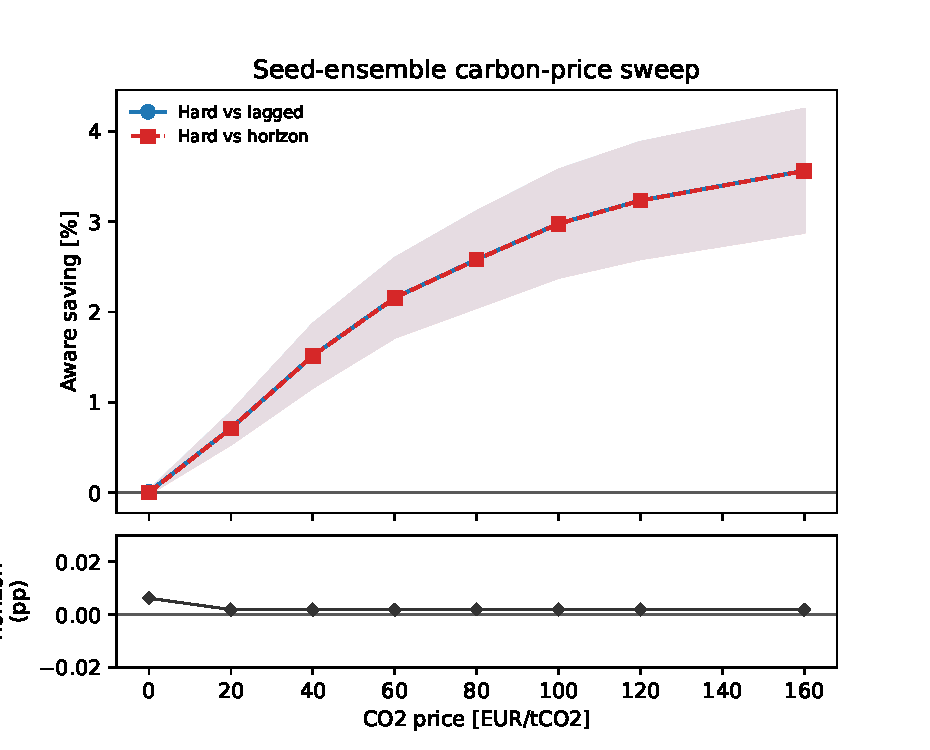
\includegraphics[width=0.88\textwidth]{fig_carbon_ensemble.pdf}
  \caption{Ten-seed carbon-price ensemble for the hard, physics-by-construction
    surrogate, Klaip\.eda Independence FSRU, 2021--2025. The main panel reports
    the five-year seed-mean aware saving against the lagged and horizon-mean
    composition baselines with 95\% confidence intervals, on a total-cost
    basis; \cref{sec:mechanism} decomposes this into volume and per-kilogram
    intensity channels. The two baselines are
    nearly indistinguishable at positive carbon prices, so the lower panel
    reports their difference in percentage points. The result is a carbon-price
    response, not a zero-carbon dispatch effect: the saving is near zero at
    $p^{\text{co2}}=0$ and rises to \lngEnsembleSavingAtOneSixZeroPct\%
    ($95\%$~CI $[\lngEnsembleCiNineFiveLoAtOneSixZeroPct,
    \lngEnsembleCiNineFiveHiAtOneSixZeroPct]$)
    at \SI{160}{\EUR\per\tCOtwo}.}
  \label{fig:carbon-ensemble}
\end{figure}

\begin{figure}[t]
  \centering
  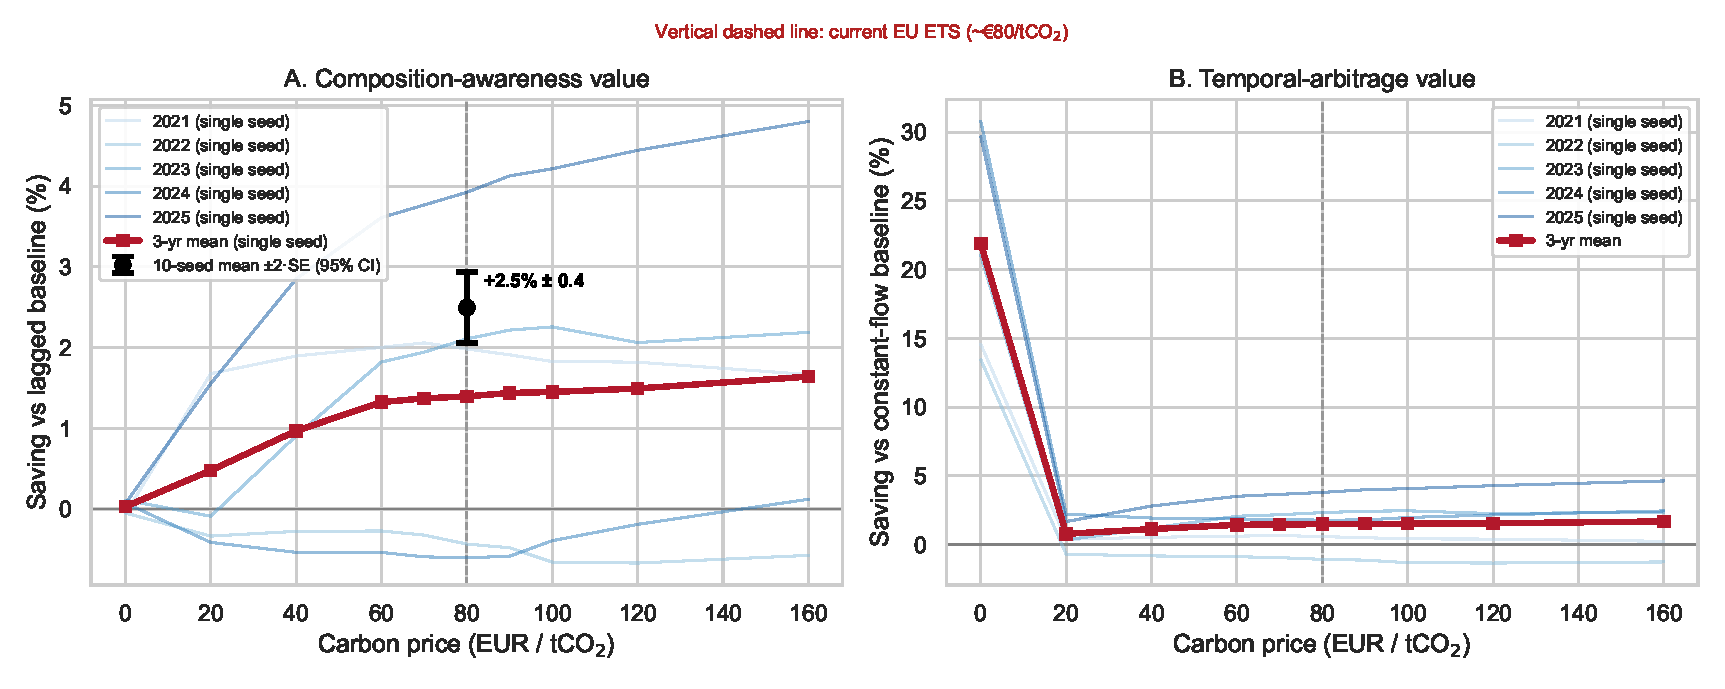
\includegraphics[width=\textwidth]{fig6_carbon_sweep.pdf}
  \caption{Single-seed and per-year companion view of composition-aware dispatch
    saving versus carbon price, Klaip\.eda Independence FSRU, 2021--2025.
    \textbf{Panel A:} saving against the lagged-composition baseline. Faint colored
    curves are single-seed sweeps for each year; the bold black line
    is the cross-year mean. Red error-bar markers at \SI{80}{\EUR\per\tCOtwo}
    show the 10-seed mean per year with 95\% CI and $\pm 2\sigma$
    intervals; these absorb the cargo-schedule variance the
    single-seed curves illustrate. \textbf{Panel B:} saving against
    the temporally optimised strategy over a constant-flow baseline, i.e. the
    value of temporal load-shifting. At zero carbon the lever yields
    \lngSingleSeedConstantFlowSavingAtZeroPct\%; at the reference carbon price
    it collapses to \lngSingleSeedConstantFlowSavingAtEightZeroPct\% because
    emissions dominate the cost denominator.
    The vertical dashed line marks \SI{80}{\EUR\per\tCOtwo}.}
  \label{fig:6_main}
\end{figure}

\begin{table}[h]
  \centering
  \caption{Seed sensitivity at \SI{80}{\EUR\per\tCOtwo}: per-year and
    $t$-tests on the null that composition-aware dispatch saves nothing
    against the lagged-composition baseline. Per-year rows use $n=10$
    cargo-schedule seeds. The five-year aggregate first averages each seed's
    five yearly saving percentages, then tests the resulting 10 seed-level
    means; the years are price regimes, not independent draws. SE is the
    standard error of the mean; 95\% CI is a Student's $t$ interval; $p$ is
    two-sided, with values below $10^{-4}$ reported as order-of-magnitude
    thresholds. The tabular is generated from
    \texttt{results/tables/seed\_significance\_hard\_co280.csv} by
    \texttt{scripts/09\_paper\_numbers.py}; a two-sided Wilcoxon signed-rank
    column appears when the regenerated artifacts carry it.}
  \label{tab:seed-significance}
  \IfFileExists{seed_significance_table.tex}{% Auto-generated by scripts/09_paper_numbers.py --write
\begin{tabular}{lrrrrrrr}
    \toprule
    Scope & $n$ & Mean (\%) & SE (\%) & 95\% CI (\%) & $t$ & $p$ & Wilcoxon $p$ \\
    \midrule
    2021 & 10 & $+4.57$ & $0.69$ & $[+3.22, +5.92]$ & $6.64$ & $<10^{-4}$ & $0.002$ \\
    2022 & 10 & $+0.89$ & $0.47$ & $[-0.02, +1.81]$ & $1.91$ & $0.088^{\dagger}$ & $0.11$ \\
    2023 & 10 & $+1.39$ & $0.39$ & $[+0.62, +2.16]$ & $3.53$ & $0.0064$ & $0.014$ \\
    2024 & 10 & $+2.54$ & $0.56$ & $[+1.44, +3.63]$ & $4.54$ & $0.0014$ & $0.0039$ \\
    2025 & 10 & $+3.52$ & $0.28$ & $[+2.97, +4.08]$ & $12.41$ & $<10^{-6}$ & $0.002$ \\
    \midrule
    \textbf{5-year mean} & \textbf{10} & $\mathbf{+2.58}$ & $\mathbf{0.27}$ & $\mathbf{[+2.05, +3.11]}$ & $\mathbf{9.56}$ & $\mathbf{<10^{-5}}$ & $\mathbf{0.002}$ \\
    \bottomrule
\end{tabular}
}{\emph{[generated table pending]}} \\[2pt]
  {\footnotesize $^{\dagger}$ Confidence interval includes zero; see \cref{sec:2022}.}
\end{table}

\subsection{Per-year structure}
\label{sec:per-year}

\Cref{fig:6_2021,fig:6_2022,fig:6_2023,fig:6_2024,fig:6_2025}
(\cref{sec:appendix-peryear}) decompose the headline number into the five
individual years, each using the two-panel layout of \cref{fig:6_main}
restricted to one year with the ten-seed mean overlaid at the
\SI{80}{\EUR\per\tCOtwo} reference value; the per-year statistics are those of
\cref{tab:seed-significance}. Read as a sequence, 2021 and the post-crisis
years carry the positive signal, 2022 is the crisis-year null
(\cref{sec:2022}), and 2024 illustrates cargo-schedule luck
(\cref{sec:2024-outlier}). 2025---the year affected by the mixed-resolution
bug, now regenerated on the corrected grid---is the tightest year. The
per-year panels are diagnostic companions rather than headline evidence; the
load-bearing claims rest on \cref{tab:seed-significance} and
\cref{fig:carbon-ensemble}.

\subsection{Supporting figures: cost delta, load-shift, volatility}
\label{sec:supporting}

The remaining figures characterise \emph{how} the aware strategy achieves its
saving, all at \SI{80}{\EUR\per\tCOtwo} on the default cargo seed.
\Cref{fig:cost_delta} shows the monthly cost delta, locating the gains in
post-cargo-arrival windows where the incoming blend differs from the
outgoing one. A per-window scatter of saving against composition variability
alone is essentially null (correlation indistinguishable from zero), so we
report that as a sentence rather than a figure: composition changes by
themselves do not generate savings; the lever appears only when those changes
coincide with economically meaningful prices and carbon factors.
\Cref{fig:load_shift} shows the flow-shift structure
behind this---deferring send-out to low-price hours for methane-rich
(low-intensity) cargoes and pulling it forward for heavier (high-intensity,
high-carbon) cargoes. Finally \cref{fig:volatility} ties the per-year
results together, showing the negative cross-year relationship between price
volatility and realised saving that underlies the 2022 null
(\cref{sec:2022}). These are single-seed visualisations: their qualitative
shape is representative across seeds, but their absolute levels are seed
42's and should be read with the caveat of \cref{sec:2024-outlier}.

\begin{figure}[htbp]
  \centering
  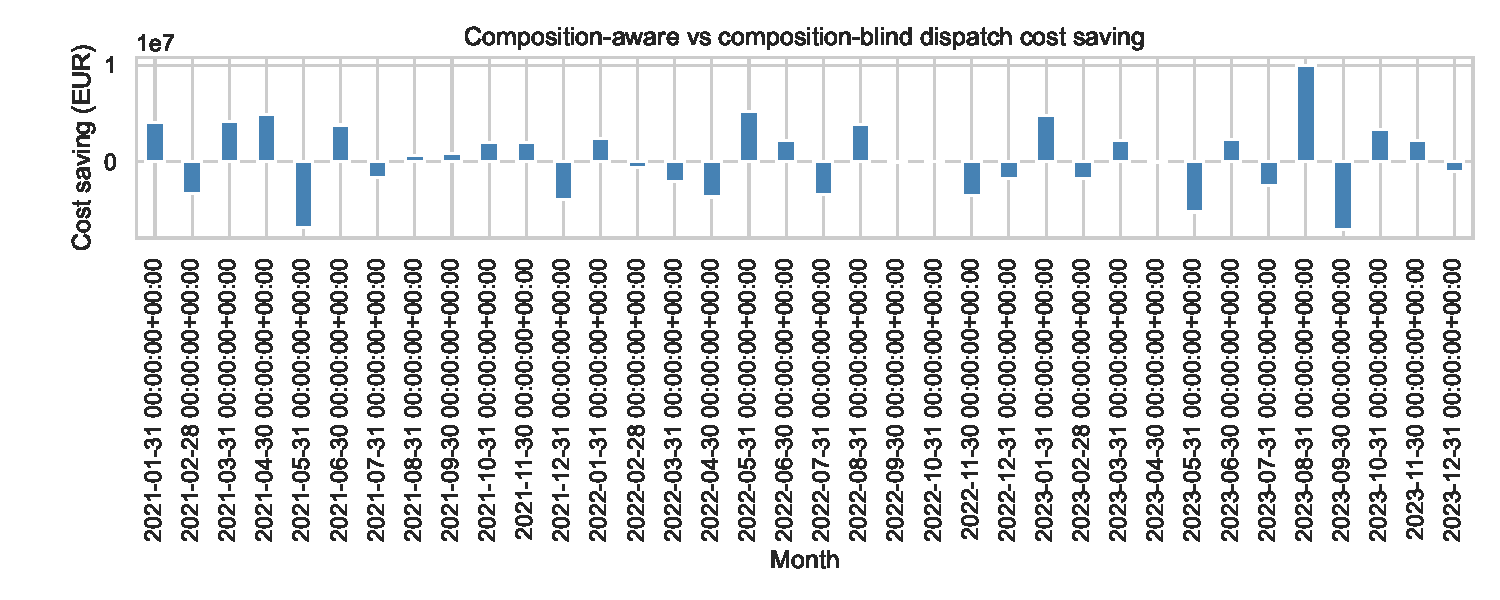
\includegraphics[width=0.95\textwidth]{fig1_cost_delta.pdf}
  \caption{Monthly cost saving from composition-aware dispatch over
    the lagged baseline, in EUR per month, single cargo realisation
    (seed~42) at \SI{80}{\EUR\per\tCOtwo}. Bars above zero indicate months
    in which the aware strategy outperformed; bars below zero indicate
    months in which the lagged strategy outperformed. The pattern
    reveals the operating regime in which the lever pays off:
    composition-rich periods (post-cargo-arrival windows where the
    incoming cargo differs materially from the previous one) carry
    most of the positive contribution. The seasonality is moderate
    and dominated by which cargo archetype the synthetic schedule
    samples in each month.}
  \label{fig:cost_delta}
\end{figure}

\begin{figure}[htbp]
  \centering
  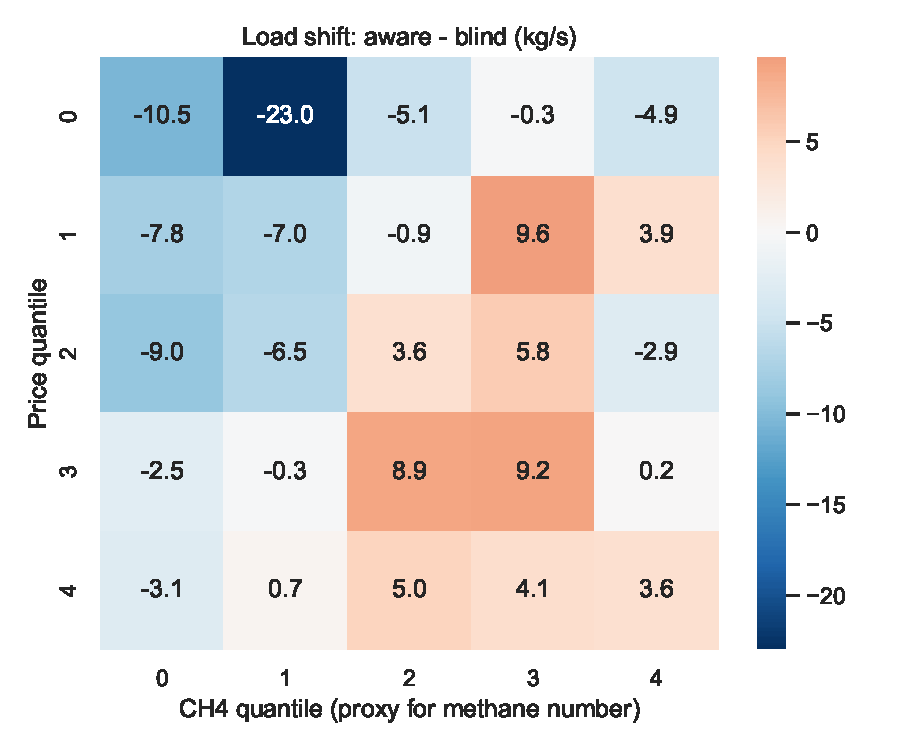
\includegraphics[width=0.85\textwidth]{fig3_load_shift.pdf}
  \caption{Hourly send-out flow shift between the aware and lagged
    strategies, binned by price quantile (x-axis) and methane number
    (y-axis). Positive cell values (red) indicate hours in which the
    aware strategy sent out \emph{more} than the lagged baseline;
    negative cells (blue) indicate the converse. The structure shows
    composition-aware dispatch deferring send-out to low-price hours
    when methane-rich cargoes are being processed (low electricity
    intensity), and pulling forward when heavier cargoes are in
    storage (high electricity intensity coupled with high carbon
    factor).}
  \label{fig:load_shift}
\end{figure}

\begin{figure}[htbp]
  \centering
  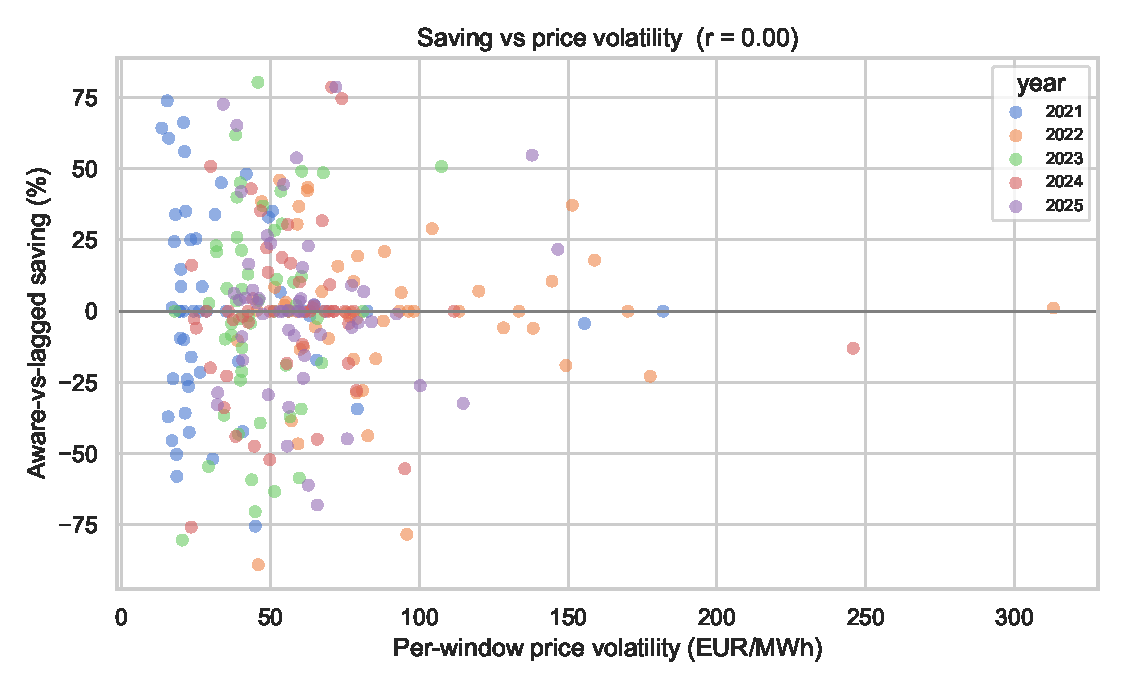
\includegraphics[width=0.85\textwidth]{fig8_volatility_vs_saving.pdf}
  \caption{Five-year relationship between per-window day-ahead price volatility
    (standard deviation of Lithuanian hourly prices, EUR/MWh) and realised
    saving from composition awareness at \SI{80}{\EUR\per\tCOtwo}. Each point is
    one 7-day dispatch window for the default cargo-schedule seed. The
    association should be read as regime structure rather than as a fitted
    mechanism: 2022 is the crisis-year null, while the normal-price years
    recover the carbon-pricing lever.}
  \label{fig:volatility}
\end{figure}

\subsection{Robustness to the tank-mixing model}
\label{sec:mixing-robustness}

The aware-versus-lagged saving is, by construction, generated entirely by the
in-tank composition transition: the lagged baseline freezes composition at the
window start, while the aware strategy tracks the blend as it evolves. If that
transition is modelled wrongly the headline number moves, and our default---a
linear blend over $\tau_{\text{mix}}=\SI{5}{\day}$---has no direct empirical
calibration. We therefore test whether the result survives plausible
alternatives. We sweep the mixing timescale over
$\tau_{\text{mix}}\in\{1,2,3,5,7,10\}~\si{\day}$ and replace the linear ramp
with a first-order (continuously-stirred-tank) kernel,
$x(t)=x_{\text{in}}+(x_0-x_{\text{in}})\,e^{-(t-t_0)/\tau_{\text{mix}}}$, which
front-loads the compositional change and is the more physically defensible
model of a stirred storage tank under continuous inflow and outflow. Both
kernels are convex combinations of the outgoing and incoming cargo and so
preserve the mole-fraction simplex exactly. The first-order kernel is
implemented in the released code and included in the manuscript artifacts. We
therefore report both the default linear-ramp sweep and the first-order CSTR
sweep, treating them as a robustness envelope rather than as calibrated tank
hydrodynamics.

The linear-ramp sweep spans \lngMixingLinearMinPct\% to
\lngMixingLinearMaxPct\% across $\tau_{\text{mix}}=\SIrange{1}{10}{\day}$,
while the CSTR sweep spans \lngMixingCstrMinPct\% to \lngMixingCstrMaxPct\%.
Every confidence interval is strictly above zero---the smallest lower bound
across all twelve cells is \lngMixingMinCiLoPct\%---so the sign of the
composition-aware saving is not an artifact of choosing a linear blend; the
two-sided Wilcoxon signed-rank test gives $\lngMixingWilcoxonMaxP$ or smaller
in every cell. All cells share the total-cost metric of \cref{sec:headline}
and therefore include the delivered-volume channel discussed in
\cref{sec:mechanism}. Under the default linear tank-mixing model, the
five-year mean saving is \lngHeadlineSavingVsLaggedPct\%. Because this
transition model generates the information gap between
the aware and lagged strategies, the result should still be interpreted as
conditional on the assumed mixing dynamics. The upper end of the sweep marks
the edge of physical plausibility: as $\tau_{\text{mix}}$ approaches the
$\approx\SI{12}{\day}$ inter-cargo interval the tank never settles between
arrivals, so $\tau_{\text{mix}}=\SI{10}{\day}$ already represents
near-continuous transition.

\begin{table}[h]
  \centering
  \caption{Five-year-mean composition-aware saving versus the lagged baseline
    at \SI{80}{\EUR\per\tCOtwo}, as a function of the tank-mixing timescale
    $\tau_{\text{mix}}$ for the default linear-ramp kernel (bold row: default
    $\tau_{\text{mix}}=\SI{5}{\day}$) and a first-order CSTR kernel. Each cell
    reports the mean saving with a $95\%$ Student's $t$ interval; the $n$
    columns report the aggregation count of the generating artifact
    (seed-first means after the corrected rerun). The tabular is generated
    from \texttt{results/tables/mixing\_table3.csv} by
    \texttt{scripts/09\_paper\_numbers.py}.}
  \label{tab:mixing-sensitivity}
  \IfFileExists{mixing_table.tex}{% Auto-generated by scripts/09_paper_numbers.py --write
\begin{tabular}{lrcrc}
    \toprule
    $\tau_{\text{mix}}$ (d) & $n$ & Linear ramp \% [95\% CI] & $n$ & First-order CSTR \% [95\% CI] \\
    \midrule
    1 & 10 & $1.60 \;[1.08, 2.12]$ & 10 & $2.03 \;[1.47, 2.60]$ \\
    2 & 10 & $1.84 \;[1.29, 2.40]$ & 10 & $2.32 \;[1.69, 2.95]$ \\
    3 & 10 & $2.20 \;[1.60, 2.80]$ & 10 & $2.47 \;[1.81, 3.13]$ \\
    \textbf{5} & 10 & $\mathbf{2.60 \;[1.91, 3.28]}$ & 10 & $\mathbf{2.61 \;[1.99, 3.23]}$ \\
    7 & 10 & $2.77 \;[2.06, 3.48]$ & 10 & $2.47 \;[1.91, 3.04]$ \\
    10 & 10 & $2.57 \;[1.83, 3.31]$ & 10 & $2.13 \;[1.68, 2.57]$ \\
    \bottomrule
\end{tabular}
}{\emph{[generated table pending]}}
\end{table}

\FloatBarrier  % flush all Results figures before Discussion begins

% =========================================================================
\section{Discussion}
\label{sec:discussion}

\subsection{Mechanism: carbon pricing makes composition matter}
\label{sec:mechanism}

% --- ADDED (carbon incidence): answers the referee's first objection --
% who actually pays phi_CO2 * m_dot? Not a standalone regas terminal under
% current ETS. Reframe p^co2 as the EFFECTIVE carbon price seen by the
% dispatching agent; name the three regimes that make it real; note the
% sweep (not the 80 EUR point) is the substantive result.
\paragraph{What the carbon term represents, and who bears it.}
The carbon cost in \cref{eq:dispatch} prices the combustion CO$_2$ of the
regasified gas, $\phi_{\text{CO}_2}(x)\,\dot m$. It is worth being explicit
that this is \emph{not} a literal model of a standalone regasification
terminal's present-day EU~ETS liability: under the current ETS the allowances
for that combustion are surrendered by the downstream emitter, not by the
terminal \citep{eu2023ets}, and with an electric trim heater the terminal's own Scope-1 footprint
is negligible. The carbon content of the trim-heater electricity, moreover, is
already internalised in $p^{\text{elec}}_t$, because EU wholesale power prices
embed the ETS cost of marginal generation; the $\phi_{\text{CO}_2}$ term
therefore captures only the throughput-combustion carbon and does not
double-count the electricity-side carbon already in the price. We accordingly
read $p^{\text{co2}}$ as the \emph{effective} carbon price faced by the
dispatching agent, and identify three regimes in which that price is non-zero
and the agent genuinely optimises against it: (i) a vertically integrated
importer-supplier whose downstream gas sales are carbon-cost-adjusted, so that
the carbon content of heavier cargoes is borne by the same balance sheet that
sets dispatch; (ii) a forward policy regime in which end-use combustion of the
delivered gas is priced---the EU ETS2 covering buildings, road transport, and
additional sectors, fully operational from 2028, with upstream fuel suppliers
as the regulated entities \citep{eu_ets2_commission_2026}, or a prospective
import-carbon charge analogous to the CBAM extended
to fossil gas---so that the carbon differential is passed back toward the point
of regasification; and (iii) an operator applying an internal or shadow carbon
price as an internal decarbonisation lever. The \SI{80}{\EUR\per\tCOtwo}
reference value is a transparent policy-sensitivity point rather than an
institutional forecast, and the substantive result is the parametric sweep of
\cref{fig:6_main}A: it reports the saving as a function of \emph{whatever}
effective carbon price the agent faces, so a reader can locate their own regime
on that axis rather than committing to ours. The upper sweep values
(\SIrange{120}{160}{\EUR\per\tCOtwo}) exceed the realised 2021--2025 ETS range
and are included as policy-sensitivity cases; \SI{80}{\EUR\per\tCOtwo} is the
reference point used for the backtest tables. Crucially, all three regimes
produce the same structural coupling---a composition-scaled cost the lagged
baseline cannot model---so the qualitative finding that carbon pricing unlocks
composition awareness is robust to the precise incidence mechanism; only the
mapping from $p^{\text{co2}}$ to a particular institution changes.

% --- DRAFT ---
% Without carbon pricing the saving in \cref{tab:seed-significance}
% collapses to zero (\cref{fig:6_main} Panel A, x = 0). This is not
% surprising in hindsight: across the operating composition envelope,
% W_total varies only $\sim 3$-$8\%$, while day-ahead prices vary by
% factors of 3-200. The optimiser has so much price arbitrage to
% capture that any composition-driven adjustment is at the margin.
%
% Adding a carbon-cost term changes the calculus. Combustion
% stoichiometry implies the emission factor $\phi_{CO_2}(x)$ ranges
% from $2.74$ kg CO_2/kg fuel for pure methane to $\sim 2.95$ for
% heavy cargoes -- a ~7\% spread that is comparable in magnitude to
% the W_total spread. The carbon cost term in \cref{eq:dispatch} thus
% adds a cost component that scales directly with cargo composition
% (not via thermodynamics) and is large in absolute EUR at EU ETS
% prices. Composition awareness becomes economically meaningful because
% it gives the optimiser information about a new, materially-sized
% cost component that the lagged baseline cannot model.
%
% This is consistent with: (i) the saving in \cref{tab:seed-significance}
% scaling with carbon price up to the EU ETS level then plateauing;
% (ii) the temporal-arbitrage saving in \cref{fig:6_main} Panel B
% collapsing from $\sim 20\%$ at zero carbon to $\sim 1\%$ at any
% positive carbon price -- once emissions are priced, the demand
% constraint pins the schedule and the temporal optimiser loses most
% of its flexibility; (iii) the volatility-conditional structure in
% \cref{fig:volatility}.

Without a carbon price the saving collapses to zero, and in hindsight this is
unsurprising. Across the operating composition envelope $W_{\text{total}}$
varies only approximately $3$--$8\%$, whereas day-ahead prices vary by factors of three
to two hundred; the optimiser has so much price arbitrage to capture that any
composition-driven adjustment is a rounding error. Adding the carbon term
changes the arithmetic. Combustion stoichiometry gives an emission factor
$\phi_{\text{CO}_2}(x)$ ranging from $2.74$~kg~CO$_2$/kg~fuel for pure
methane to approximately $2.95$ for heavy cargoes---an approximately $7\%$ spread,
comparable in magnitude to the $W_{\text{total}}$ spread but, crucially,
priced at reference carbon-price levels where it is large in absolute euros and scales
directly with composition rather than through the thermodynamics. Carbon
pricing thus hands the optimiser a new, materially sized cost component that
the lagged baseline cannot model, and composition awareness becomes
economically meaningful. Once emissions are priced, the carbon term becomes
the dominant component of total cost. Part of the observed decline in
percentage temporal-arbitrage value is therefore mechanical: the denominator
increases even when the absolute electricity-arbitrage value changes little.
Three observations corroborate this mechanism: the saving scales with carbon
price up to the reference range and then plateaus (\cref{fig:6_main}A); the
temporal-arbitrage percentage saving declines once the carbon term dominates
the cost denominator (\cref{fig:6_main}B); and the per-window saving is
concentrated where composition transitions coincide with material prices and
carbon factors (\cref{fig:cost_delta}) rather than tracking composition
variability alone.

\paragraph{Volume versus intensity: what the saving is made of.}
The post-processing decomposition
(\texttt{scripts/16\_cost\_decomposition.py}) replays the committed schedules
against the realised composition trajectory and splits each seed's
aware-versus-lagged saving along two axes. Along the first
axis---electricity versus carbon---the carbon term carries approximately
\lngDecompCarbonSharePct\% of the saving, with the electricity term slightly
adverse. The second axis is the consequential one. The aware schedule realises
\lngDecompDeliveredMassDeltaPct\% delivered mass relative to the lagged
baseline, and the per-year total-cost saving tracks this volume difference
almost one-for-one. The mechanism is a design property of the rolling
horizon: the contracted-demand constraint binds within each seven-day
\emph{plan}, but only the first \SI{24}{\hour} of each plan are committed, so
realised annual send-out can drift between strategies---and a
composition-aware optimiser facing a carbon-dominated bill systematically
defers more volume than its composition-blind counterpart. Volume-matched,
the comparison shrinks by two orders of magnitude: the per-kilogram cost
saving is \lngDecompSavingPerKgPct\% ($95\%$~CI
$[\lngDecompPerKgCiNineFiveLoPct, \lngDecompPerKgCiNineFiveHiPct]$, all ten
seeds positive) and the per-kilogram carbon-intensity improvement is
\lngDecompCoTwoIntensitySavingPct\%. The realised emission difference of
\num{\lngDecompMeanCoTwoSavingT}~\si{\tCOtwo} per seed-year is likewise
volume-dominated and should not be read as abatement: gas the model does not
send out is demand deferred, not demand destroyed. The honest reading of the
headline is therefore an intensity effect that is statistically robust but
economically small, plus a volume-shift effect whose value depends entirely
on how undelivered volume is treated contractually. The decisive robustness
check removes the volume channel by construction, and we implement it as a
volume-matched backtest mode (\texttt{--volume-matched}): each window's
demand becomes the contract-to-date shortfall---rolling volume-debt
accounting, since a per-plan equality alone would still let a strategy
back-load every plan---and total send-out is capped at $0.1\%$ above that
shortfall. The matching works: the pooled realised delivered-mass difference
drops to \lngVolmatchDeliveredMassDeltaPct\% (at most
\lngVolmatchMaxAbsYearMassDeltaPct\% in any single year, the wobble of
slicing a continuously debt-tracked five-year run at year boundaries). In the
volume-matched run, the aware-versus-lagged saving is \lngVolmatchSavingPct\%
($95\%$~CI $[\lngVolmatchCiNineFiveLoPct, \lngVolmatchCiNineFiveHiPct]$,
$\lngVolmatchPTwoSided$, Wilcoxon $\lngVolmatchWilcoxonPTwoSided$,
$n=\lngVolmatchSeedN$, all seed means positive)---somewhat above the
per-kilogram replay estimate, because the constrained optimiser redirects
composition information from volume-shedding into timing. No individual year
is significant on its own; only the pooled five-year mean is, which is the
signature of an effect that is consistent but small. This number, not the
total-cost headline, is the per-unit value of composition awareness.

\subsection{2022: the energy-crisis null}
\label{sec:2022}

% --- DRAFT ---
% 2022 is the only year in which the headline test fails to reject the
% null at the conventional $p = 0.05$ threshold ($p = 0.088$,
% \cref{tab:seed-significance}). The mechanism is the inverse of
% \cref{sec:mechanism}: when electricity prices are so high that
% temporal arbitrage dominates the dispatch, composition awareness
% loses its leverage because every hour is already constrained by
% price timing. The single-seed trajectory in \cref{fig:6_2022}
% remains slightly negative across all positive carbon prices; the
% seed mean is just barely positive but its CI includes zero. We
% report this as a regime-conditional null rather than treating it as
% a generalisation failure: composition awareness works reliably in
% normal-price years and is operationally irrelevant during extreme
% price events. This is itself a result of operational interest --
% terminal operators can rely on the lever in stable price regimes
% but should not expect it to compensate for crisis-period electricity
% costs.

2022 is the only year in which the test fails to reject the no-saving null at
the conventional threshold ($p=0.088$, \cref{tab:seed-significance}). The
year is also statistically underpowered for small positive effects: with the
2022 standard error of \cref{tab:seed-significance} ($\approx 0.5$ percentage
points) and $n=10$ seeds, a two-sided $\alpha=0.05$ test has only roughly
$50\%$ power against a true $+1$ percentage-point saving. We therefore read 2022 as a regime-specific weak
or null result, not as proof that the effect is exactly zero. The
mechanism is the mirror image of \cref{sec:mechanism}: when electricity
prices are extreme, temporal arbitrage dominates the dispatch and every hour
is already tightly constrained by price timing, so composition awareness has
no slack left to exploit. \Cref{fig:volatility} makes this visible---realised
saving falls as price volatility rises---and \cref{fig:6_2022} shows the
single-seed trajectory sitting slightly negative across all carbon prices,
with the seed mean barely positive and its CI straddling zero. We frame this
as a regime-conditional null rather than a generalisation failure:
composition awareness is a reliable lever in normal-price years and is simply
not distinguishable from the lagged baseline during an extreme price event.
That is itself operationally useful---an operator can lean on the lever in
normal regimes but should not expect it to offset crisis-period electricity
costs.

\subsection{2024 outlier: cargo-schedule luck and why we report the seed mean}
\label{sec:2024-outlier}

In \cref{fig:6_2024} the default-seed sweep sits essentially at zero across
positive carbon prices, yet the ten-seed mean is robustly positive
(\cref{tab:seed-significance}). The seed-level breakdown in
\cref{sec:appendix-seeds} shows the same pattern: in 2024 the default seed is
the lowest of the ten cargo realisations and lies far below the seed mean,
and in 2021 it is also near the bottom of the distribution. The reading
is mundane but important---cargo schedules are stochastic and a single
realisation can be unlucky in a given year, which is exactly the variance the
seed protocol (\cref{sec:seed-protocol}) exists to absorb. We therefore
report the seed mean with its confidence interval, never the single-seed
number, as each year's result. The single-seed sweep \emph{curves} remain
useful as illustrations of how the saving responds to carbon price, but
should not be read as point predictions for a specific terminal-year.

\subsection{Surrogate controls: no material soft-only artifact detected}
\label{sec:methodological-warning}

The soft-vs-hard comparison is a control, not the paper's main contribution. It
tests whether the dispatch result depends on an architecture-specific surrogate
artifact: two
surrogates are trained on identical data, seeds, and optimisation budget---one
with the conventional
soft-physics recipe \citep{raissi2019physics}, predicting $W_{\text{pump}}$,
$W_{\text{total}}$, $T_{\text{out}}$, and exergy jointly with soft energy- and
mass-balance penalties, and one with the physics-by-construction architecture of
\cref{sec:pinn}---and the identical ten-seed dispatch backtest is run with each at
$p_{\text{co}_2}\in\{0, \SI{80}{\EUR\per\tCOtwo}\}$. The test is negative in
the released artifacts. Against the lagged baseline, the hard surrogate reports
\lngSvhHardAtZeroMeanPct\% ($95\%$~CI $[\lngSvhHardAtZeroCiNineFiveLoPct,
\lngSvhHardAtZeroCiNineFiveHiPct]$) at zero carbon and
\lngSvhHardAtEightZeroMeanPct\% ($95\%$~CI
$[\lngSvhHardAtEightZeroCiNineFiveLoPct,
\lngSvhHardAtEightZeroCiNineFiveHiPct]$) at \SI{80}{\EUR\per\tCOtwo}; the
corresponding soft-surrogate values are \lngSvhSoftAtZeroMeanPct\%
($95\%$~CI $[\lngSvhSoftAtZeroCiNineFiveLoPct,
\lngSvhSoftAtZeroCiNineFiveHiPct]$) and \lngSvhSoftAtEightZeroMeanPct\%
($95\%$~CI $[\lngSvhSoftAtEightZeroCiNineFiveLoPct,
\lngSvhSoftAtEightZeroCiNineFiveHiPct]$). The soft-minus-hard contrast is only
\lngSvhContrastAtZeroPp{} percentage points at zero carbon and
\lngSvhContrastAtEightZeroPp{} percentage points at \SI{80}{\EUR\per\tCOtwo}.
A separate fabrication diagnostic over \lngFabSeedCount{} seeds and
\lngFabWindowsPerSeed{} validation windows per seed flags
\lngFabHardFlaggedWindows{} windows for the hard and
\lngFabSoftFlaggedWindows{} for the soft model. We therefore do not claim that
the trained soft surrogate fabricated the headline dispatch signal; the result
is instead that the diagnostic successfully rules out a material soft-only
artifact under this training protocol.

The potential failure mode would be an asymmetric error structure. The aware
strategy queries the surrogate at a composition that
varies hour to hour, while the lagged strategy queries at a single fixed
composition; any composition-dependent bias in a surrogate can therefore become a
\emph{systematic} differential cost between the two strategies rather than
averaging out. Such a bias can be negligible in held-out accuracy while still
being comparable to the economic effect under study, and can survive directly
into the reported saving. The hard-constrained
architecture removes them by construction, because the cost-determining channel is
tied to exact thermodynamics and depends on the network only through a single
bounded scalar. This is distinct from the prediction-accuracy case for hard
constraints made elsewhere
\citep{krishnapriyan2021characterizing,chalapathi2024moe,chen2024kkt}: the bias
here is invisible to accuracy and manifests only in the \emph{decision}.

The diagnostic generalises to any pipeline that uses a learned surrogate to
compare decisions querying different regions of the input space. For each
surrogate, compute the cost difference between
a time-varying composition trajectory and its window-mean composition, then
compute the same difference from the ground-truth simulator; their discrepancy
is a fabrication diagnostic. As a deliberately conservative heuristic, if the
surrogate-only difference exceeds the simulator difference by more than roughly
$1$--$2\%$ of the simulator cost---about half the headline effect size in the
reference run---the architecture is creating signal and must not be placed
inside an optimiser without hard constraints or on-trajectory validation. In
the present run this check stays well below that threshold for both
architectures.

\subsection{Limitations}
\label{sec:limitations}

% --- DRAFT ---
% \textbf{Single terminal.} Results are for one FSRU configuration
% (ORV + trim heater, Klaip\.eda layout). Different topologies
% (e.g. submerged combustion vaporiser, ambient air vaporiser) would
% shift the relative importance of trim-heater electricity vs.
% seawater heat, changing the surrogate's input-output structure and
% thus the absolute saving. The methodology is portable; the
% headline number is not.
%
% \textbf{Single bidding zone.} 2021--2025 Lithuanian DA prices.
% Generalisation to other zones (DE\_LU, NL, IT) is straightforward
% with the v1.5 site-aware data pull but was not pursued; we expect
% the qualitative shape of \cref{fig:6_main} to hold but the
% per-year coefficients to shift.
%
% \textbf{Synthetic cargo schedule.} Composition trajectories are
% derived from GIIGNL archetype mole fractions with a probabilistic
% inter-cargo schedule. Real FSRU operators have access to assayed
% composition data per cargo; replacing the synthetic schedule with
% real terminal data would tighten the per-year confidence intervals
% but is not expected to change the headline mechanism.
%
% \textbf{Steady-state plant model.} The CoolProp ground truth is
% steady-state per operating point; transient effects (cargo
% transfer, tank cooldown) are not modelled. For hourly dispatch
% decisions this is conventional, but it limits applicability to
% sub-hourly optimisation.
%
% \textbf{Surrogate fidelity vs.\ ground-truth.} The PINN matches
% CoolProp to median relative cost error $< 10^{-4}$ on the dispatch
% trajectory, but CoolProp's HEOS backend itself has accuracy
% limitations for heavy hydrocarbons near critical conditions
% (\citet{bell2014pure}). The surrogate inherits these.

Several limitations bound the scope of these results.
\textbf{Single terminal:} we model one FSRU configuration (ORV plus trim
heater, the Klaip\.eda layout). Other topologies---submerged-combustion or
ambient-air vaporisers---would shift the balance between trim-heater
electricity and free seawater heat, altering the surrogate's input--output
structure and the absolute saving; the methodology ports directly, but the
headline number does not. More generally, the workflow ports to other
vaporiser topologies, climates, and market zones, but the numerical savings
reported here are Klaip\.eda-specific. \textbf{Single bidding zone:} we use 2021--2025
Lithuanian day-ahead prices. The v1.5 data layer is site-aware and a
second-zone study (DE\_LU, NL, IT) is mechanically straightforward but was
not pursued here; we expect the qualitative shape of \cref{fig:6_main} to
carry over with shifted per-year coefficients. \textbf{Synthetic cargo
schedule:} composition trajectories use GIIGNL archetype mole fractions with
a probabilistic arrival schedule. Real terminals have assayed per-cargo
composition; substituting it would tighten the per-year confidence intervals
but should not change the mechanism. The composition range is limited to the
GIIGNL archetypes and the LHS training envelope; extrapolation to unseen cargo
qualities is not claimed. \textbf{Tank-mixing dependence:} the
aware-versus-lagged information gap is generated by the assumed in-tank
transition; \cref{sec:mixing-robustness} bounds this with two kernels and six
timescales but does not calibrate it against tank hydrodynamics.
\textbf{Oracle foresight:} the aware
strategy knows the true blended composition over the full horizon, so the
saving is an upper bound on deployable composition forecasting.
\textbf{Volume non-equivalence:} under the floor-only demand model the
realised annual delivered mass differs between compared strategies
(\lngDecompDeliveredMassDeltaPct\%; \cref{sec:mechanism}), so total-cost
savings mix a dominant volume channel with a small per-kilogram intensity
channel, and revenue forgone on undelivered volume is not modelled. The
volume-matched mode of \cref{sec:mechanism} removes this channel by
construction and supplies the per-unit number.
\textbf{Steady-state plant model:} the
CoolProp ground truth is steady-state per operating point and omits
transients (cargo transfer, tank cooldown); this is conventional for hourly
dispatch but limits sub-hourly applicability. \textbf{Simulator dependence and
plant validation:} the surrogate is validated against CoolProp, not against
plant operating data. \textbf{Inherited thermodynamic error:} the surrogate matches CoolProp to a
median absolute relative cost error of \num{\lngFidelityMedianAbsRelError} on
the trajectory, but the HEOS backend itself is less
accurate for heavy hydrocarbons near critical conditions
\citep{bell2014pure}, and the surrogate inherits that. \textbf{Uncertainty:}
the reported p-values quantify variability over the synthetic cargo-schedule
generator only. They do not propagate market prices, demand, weather, terminal
controls, property-model uncertainty, plant measurements, or cargo assay data.
The results should therefore be interpreted as controlled simulation evidence
for a carbon-pricing scheduling mechanism rather than as an audited estimate of
real terminal savings.

% =========================================================================
\section{Conclusion}
\label{sec:conclusion}

This paper now has a narrower and more defensible message. The operational
question is whether knowing LNG cargo composition helps an FSRU operator
dispatch more cheaply. On the corrected uniform-hourly data the answer is
conditional on an effective carbon price, driven by closed-form combustion
stoichiometry---and, decisively, structured by delivered volume: almost all of
the \lngHeadlineSavingVsLaggedPct\% total-cost saving against the lagged
baseline reflects the aware schedule realising
\lngDecompDeliveredMassDeltaPct\% delivered mass under the rolling demand
floor, while a volume-matched rerun of the dispatch puts the per-unit saving
at \lngVolmatchSavingPct\%. Composition awareness is thus a small but
statistically robust carbon-intensity lever plus a larger volume-shift effect
whose value depends on the contractual treatment of undelivered volume. The
neural surrogate is not the source of the economic result. It remains valuable
as a fast way to include the plant electricity term in repeated
rolling-horizon optimisation, but the decomposition shows the saving is
carried by the carbon term, with electricity slightly adverse.

The soft-vs-hard experiment should therefore be read as a control. It falsifies
the stronger methods story: the trained soft surrogate does not fabricate a
material composition-saving signal relative to the physics-by-construction
surrogate, with soft-minus-hard contrasts of at most \lngSvhMaxAbsContrastPp{}
percentage points and \lngFabHardFlaggedWindows{} (hard) and
\lngFabSoftFlaggedWindows{} (soft) flagged fabrication windows in the current
artifacts. The practical
message is consequently simpler: once volume is matched, composition-aware
dispatch is a small simulated carbon-pricing lever, and the pipeline reports
it as such. An equality-constrained (fixed-volume) dispatch comparison, real
assayed cargo data, additional bidding zones, alternative vaporiser
topologies, and calibrated tank mixing remain the natural path to a
submission-ready applied-energy paper.

% =========================================================================
\section{Reproducibility}
\label{sec:repro}

\textbf{Code and data.} The full pipeline is available at
\url{https://github.com/Zorkendorfer/lng-pinn}. The results reported here were
generated with Python~3.11, dependencies pinned by \texttt{pyproject.toml} and
\texttt{uv.lock}, and the trained checkpoint \texttt{results/models/pinn\_v1.pt}.
The run metadata and expected artifact list are recorded in
\texttt{results/tables/run\_manifest.json}. The independent cargo-schedule seeds
are \texttt{42, 0, 1, 7, 13, 19, 23, 31, 37, 53}. The ENTSO-E token used to fetch
day-ahead prices is read from \texttt{.env}; processed price/weather/cargo tables
and generated results are written under \texttt{data/processed/},
\texttt{results/tables/}, and \texttt{results/figures/}.

\textbf{Reproducing the headline number.} From a clean clone with the ENTSO-E
token configured, the low-level rebuild path is:
\begin{verbatim}
uv run python scripts/01_pull_entsoe.py --start 2021-01-01 \
    --end 2026-01-01 --zone LT
uv run python scripts/02_build_dataset.py
uv run python scripts/18_audit_artifacts.py --timeseries-only --strict
uv run python scripts/03_train_pinn.py --no-resume --lambda-c 1.0
\end{verbatim}
The paper-level rework phases then regenerate the result tables, robustness
diagnostics, figures, and manifest:
\begin{verbatim}
./run_rework.sh cstr
./run_rework.sh soft
./run_rework.sh fabrication
./run_rework.sh ensemble
./run_rework.sh manifest
./run_rework.sh volmatch
\end{verbatim}
The \texttt{manifest} phase refreshes figures, writes the run manifest, runs the
cheap decomposition and $T_{\text{out}}$ audits, regenerates paper-number
macros, and performs the artifact audit. The \texttt{volmatch} phase runs the
volume-matched comparison of \cref{sec:mechanism}
(\texttt{06\_seed\_sensitivity.py --volume-matched}, tagged
\texttt{hard\_volmatch} so it never collides with the floor-constraint
artifacts) and replays its cost decomposition. The manuscript itself contains no
hand-typed result digits: prose values resolve from
\texttt{paper/paper\_macros.tex} and the result tables are generated includes
(\texttt{seed\_significance\_table.tex}, \texttt{mixing\_table.tex},
\texttt{surrogate\_eval\_table.tex}), all written by
\texttt{scripts/09\_paper\_numbers.py --write}, so a pipeline rerun refreshes
every quantitative claim in one step.
The long-running phases can also be batched through
\texttt{run\_rework\_overnight.sh}. The underlying commands for the reference
10-seed sensitivity and carbon ensemble are:
\begin{verbatim}
uv run python scripts/06_seed_sensitivity.py --no-resume \
    --carbon-price 80 --workers 10 --validation-sample-frac 0.05
uv run python scripts/13_carbon_ensemble.py \
    --prices 0 20 40 60 80 100 120 160 --strict
\end{verbatim}
The tank-mixing sweep is run separately with
\begin{verbatim}
uv run python scripts/09_mixing_sensitivity.py --carbon-price 80 --workers 10
uv run python scripts/14_mixing_table.py --strict
\end{verbatim}
and writes \texttt{results/tables/mixing\_sensitivity.csv} and
\texttt{results/tables/mixing\_table3.csv} when complete. The
surrogate-speed benchmark is intentionally separated from the manuscript build:
\begin{verbatim}
uv run python scripts/10_benchmark_speed.py
\end{verbatim}
It performs the requested 10,000 CoolProp HEOS calls and 10,000 surrogate
forward passes on the same sampled operating points.
For a smaller CSV-emitting benchmark with hardware metadata, run:
\begin{verbatim}
uv run python scripts/10_benchmark_surrogate.py --n 500
\end{verbatim}
This writes \texttt{results/tables/speed\_benchmark.csv}.

\appendix
\section{Per-year carbon-sweep companions}
\label{sec:appendix-peryear}

Each panel repeats the layout of \cref{fig:6_main} for a single year: the blue
curve traces the aware-versus-lagged saving for the default cargo schedule
(seed~42) as the effective carbon price varies, and the red marker at
\SI{80}{\EUR\per\tCOtwo} shows the ten-seed mean with its $95\%$ confidence
interval. The per-year means, intervals, and test statistics are those of
\cref{tab:seed-significance}; the single-seed curves illustrate cargo-schedule
variance and are not the reported per-year results.

\begin{figure}[htbp]
  \centering
  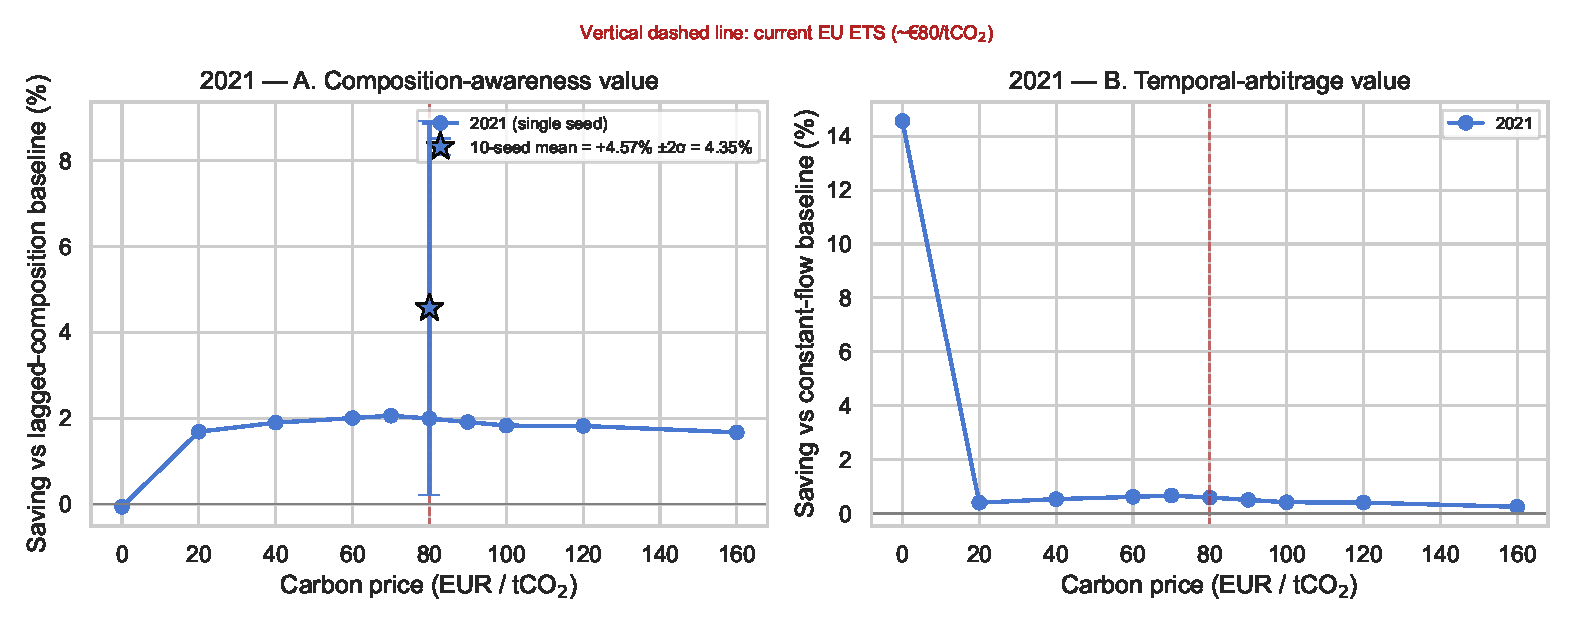
\includegraphics[width=\textwidth]{fig6_carbon_sweep_2021.pdf}
  \caption{2021 companion. The strongest year: every cargo realisation is
    positive, with wide seed variance reflecting the headroom the lever has
    when electricity prices are at normal pre-crisis levels.}
  \label{fig:6_2021}
\end{figure}

\begin{figure}[htbp]
  \centering
  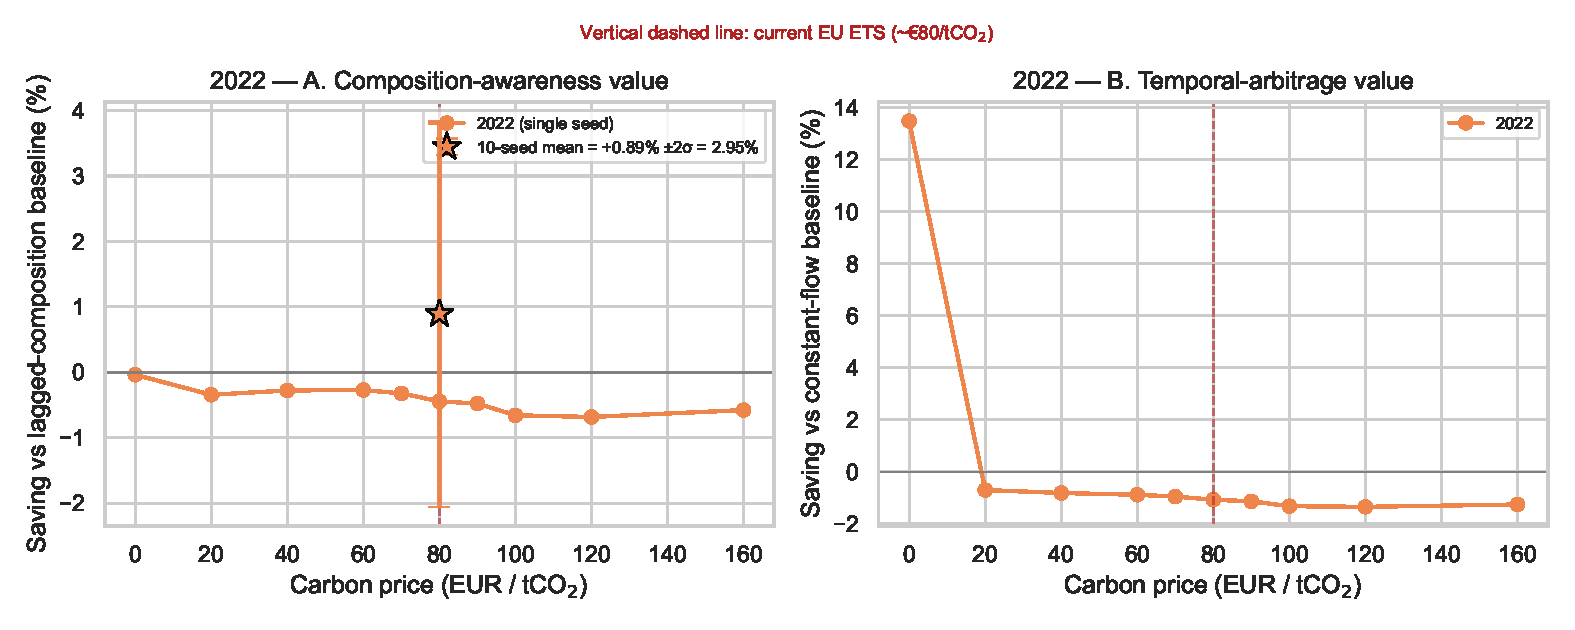
\includegraphics[width=\textwidth]{fig6_carbon_sweep_2022.pdf}
  \caption{2022 companion. The European energy-crisis year: the
    default-seed trajectory sits slightly negative across carbon prices and
    the ten-seed mean straddles zero, the regime-conditional null discussed in
    \cref{sec:2022}.}
  \label{fig:6_2022}
\end{figure}

\begin{figure}[htbp]
  \centering
  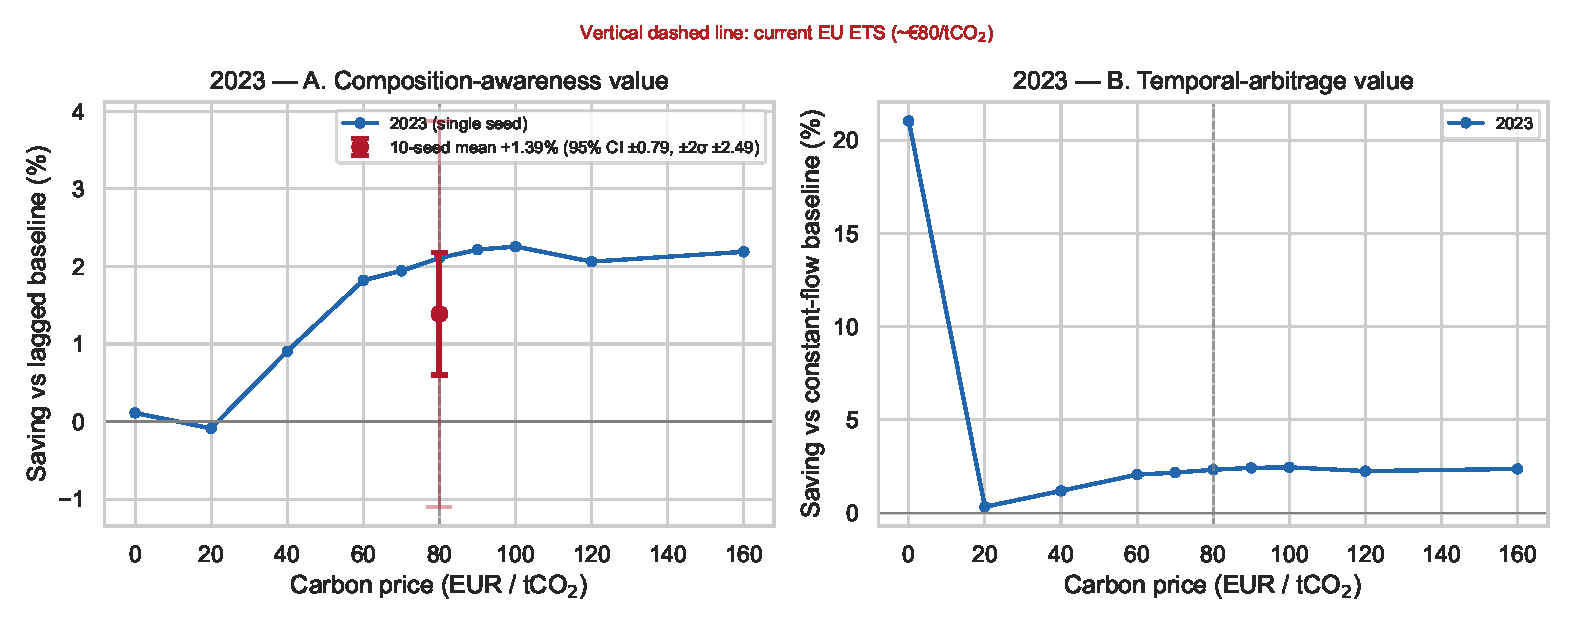
\includegraphics[width=\textwidth]{fig6_carbon_sweep_2023.pdf}
  \caption{2023 companion. Post-crisis recovery year: positive at the seed
    mean, though with a wider spread across cargo realisations than 2021's
    all-positive pattern, including two negative realisations.}
  \label{fig:6_2023}
\end{figure}

\begin{figure}[htbp]
  \centering
  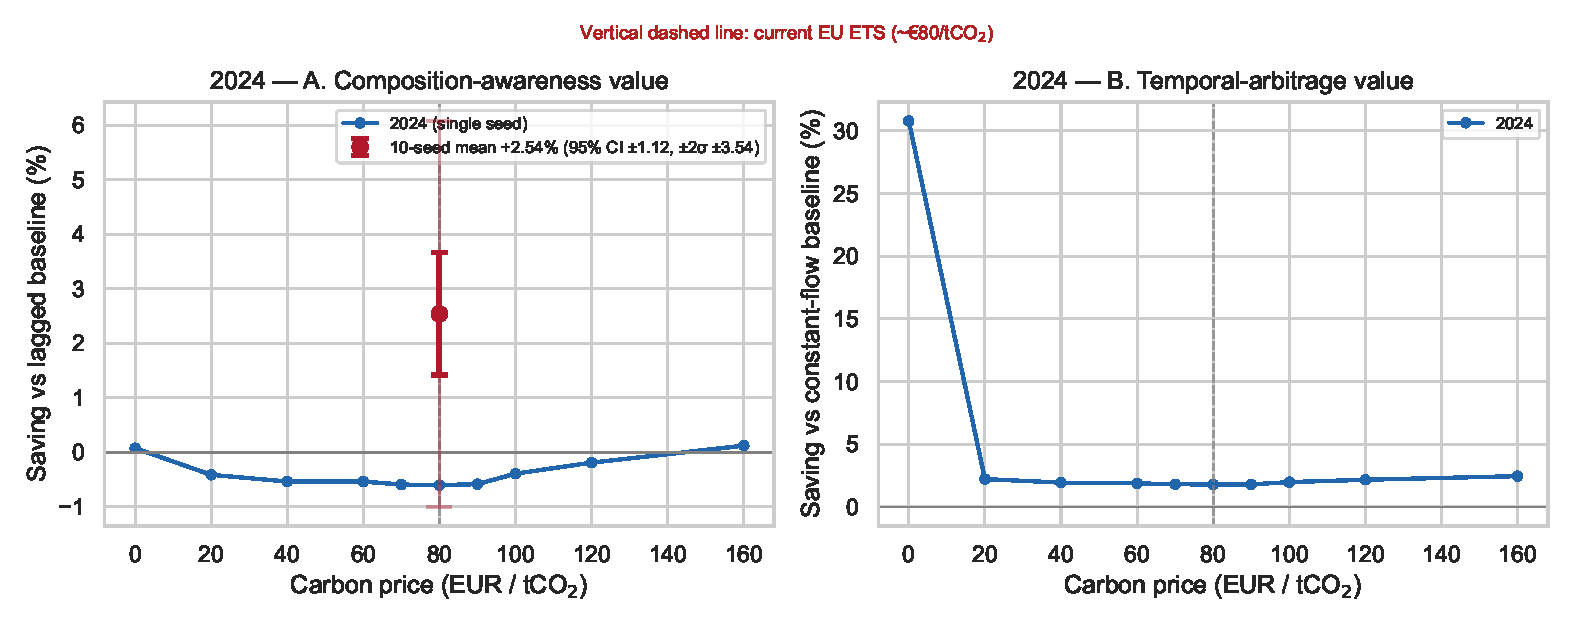
\includegraphics[width=\textwidth]{fig6_carbon_sweep_2024.pdf}
  \caption{2024 companion. The default seed is the lowest of the ten
    realisations, sitting near zero while the seed mean is robustly
    positive---the clearest illustration of why the seed mean, not a single
    realisation, is the reported quantity (\cref{sec:2024-outlier}).}
  \label{fig:6_2024}
\end{figure}

\begin{figure}[htbp]
  \centering
  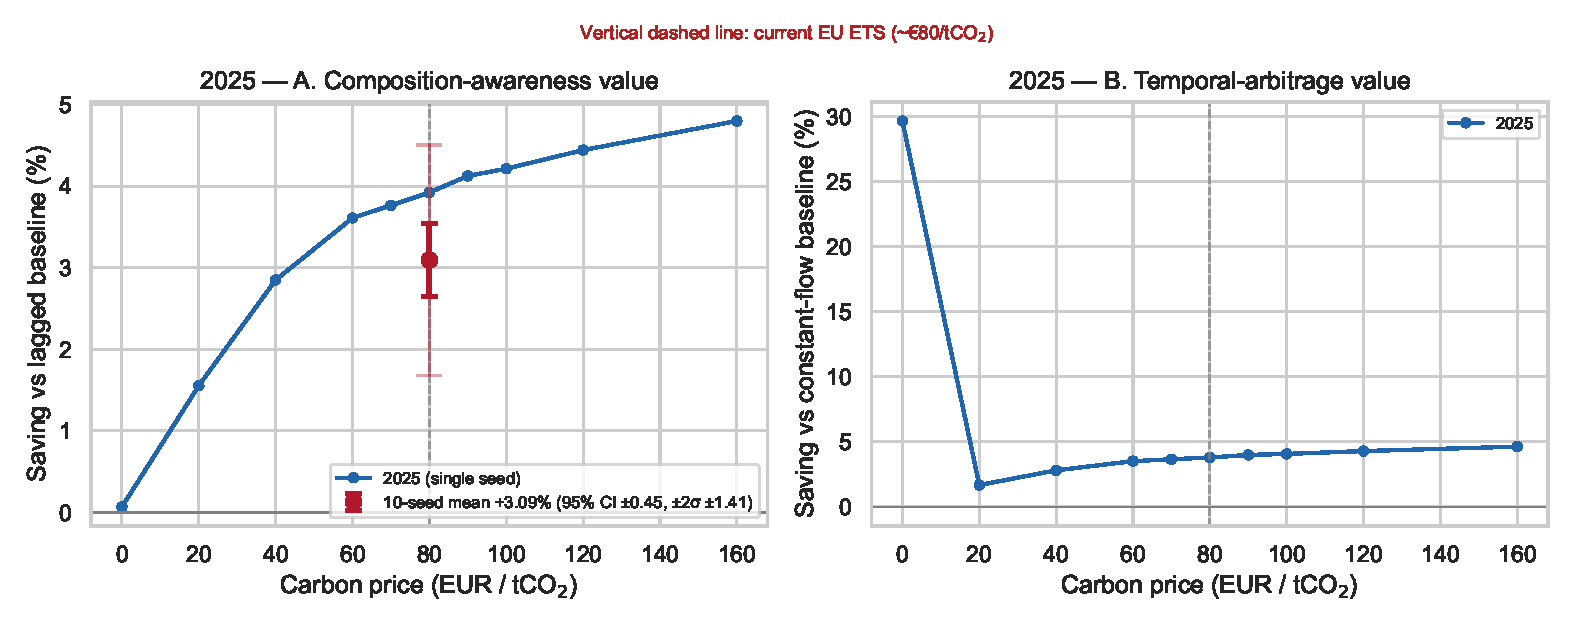
\includegraphics[width=\textwidth]{fig6_carbon_sweep_2025.pdf}
  \caption{2025 companion. This is the year that was contaminated by
    mixed-resolution settlement rows in the superseded timeseries; the panel
    shown here is regenerated on the corrected uniform-hourly grid, on which
    2025 is the tightest and most significant year
    (\cref{tab:seed-significance}).}
  \label{fig:6_2025}
\end{figure}

\FloatBarrier

\section{Seed-level sensitivity}
\label{sec:appendix-seeds}

% Auto-generated by scripts/09_paper_numbers.py --write
\begin{table}[h]
  \centering
  \caption{Composition-aware saving versus the lagged-composition baseline by cargo-schedule seed and year at \SI{80}{\EUR\per\tCOtwo}. Values are percentages.}
  \label{tab:seed-supplement}
  \begin{tabular}{rrrrrr}
    \toprule
    Seed & 2021 & 2022 & 2023 & 2024 & 2025 \\
    \midrule
    0 & +3.90 & -0.34 & +2.03 & +3.02 & +3.11 \\
    1 & +5.47 & +0.59 & +1.89 & +3.78 & +3.64 \\
    7 & +6.37 & +0.25 & +0.45 & +1.53 & +2.68 \\
    13 & +1.85 & +0.40 & +2.41 & +5.32 & +1.91 \\
    19 & +4.57 & +3.28 & -0.28 & +1.89 & +4.07 \\
    23 & +7.78 & +1.46 & +2.88 & +1.75 & +3.65 \\
    31 & +1.72 & +0.03 & -0.96 & +3.50 & +2.76 \\
    37 & +5.16 & -0.01 & +1.91 & +0.89 & +2.77 \\
    42 & +1.98 & -0.43 & +2.11 & -0.60 & +3.93 \\
    53 & +6.86 & +3.71 & +1.43 & +4.31 & +2.43 \\
    \bottomrule
  \end{tabular}
\end{table}


% =========================================================================
\clearpage  % ensure no deferred float lands among the references
\bibliographystyle{plainnat}
\bibliography{refs}

\end{document}
